% !TeX program = xelatex
% !TeX encoding = UTF-8 Unicode
% !BIB program = biber

\documentclass[ieee,english]{slides}

\DeclareMathOperator*{\argmax}{arg\,max}
\DeclareMathOperator*{\argmin}{arg\,min}
\newcommand{\norm}[1]{\left\lVert#1\right\rVert}
\newcommand{\cmark}{\ding{51}}
\newcommand{\xmark}{\ding{55}}
\newcommand{\adj}{\textrm{adj}}
\newcommand{\tr}{^{\top}}
\renewcommand{\bar}[1]{\overbar{#1}}
\newcommand{\ubar}[1]{\underbar{#1}}

\title{Surveillance distribuée des systèmes cyber-physiques:\\application aux usines intelligentes}

\addauthor{Álan Crístoffer e Sousa}{alan.e-sousa@univ-reims.fr}

\setorientador{Prof.\ Dr.\ Nadhir Messai}
\addcoorientador{Prof.\ Dr.\ Noureddine Manamanni}

\setdepartamento{CReSTIC}
\seteixodeformacao{Automation and Signal Processing}

\setlocal{Reims}
\setano{2022}
\setmes{July}

\preamble{}
\input{colors}

\addbibresource{bibliothek.bib}
\graphicspath{{imgs/}}%

\newcommand{\y}{\textcolor{flame}{\ensuremath{y(t)}}}
\newcommand{\z}{\textcolor{red}{\ensuremath{z(t)}}}
\newcommand{\w}{\textcolor{auburn}{\ensuremath{w(t)}}}
\newcommand{\hz}{\textcolor{red}{\ensuremath{\hat{z}(t)}}}
\newcommand{\dw}{\textcolor{auburn}{\ensuremath{\dot{w}(t)}}}
\newcommand{\mN}{\textcolor{frenchblue}{\ensuremath{N}}}
\newcommand{\mJ}{\textcolor{frenchblue}{\ensuremath{J}}}
\newcommand{\mH}{\textcolor{frenchblue}{\ensuremath{H}}}
\newcommand{\mE}{\textcolor{frenchblue}{\ensuremath{E}}}

\newcommand{\cubar}[1]{\textcolor{frenchblue}{\ubar{#1}}}
\newcommand{\cbar}[1]{\textcolor{flame}{\bar{#1}}}

\begin{document}
\maketitle{}

\begin{slide}{Index}
  \begin{minipage}[t][0.4\textheight][t]{0.45\textwidth}
    \tableofcontents[sections={1-4}]
  \end{minipage}
  \begin{minipage}[t][0.4\baselineskip][t]{0.45\textwidth}
    \tableofcontents[sections={5-}]
  \end{minipage}
  \vfill\null{}
\end{slide}

% !TeX root = document.tex
% !TeX encoding = UTF-8 Unicode

\section{Introduction}%
\label{sec:introduction}

\begin{slide}{Attacks on Dynamic Systems}
  \begin{columns}[c]
    \begin{column}{0.48\textwidth}
      \begin{itemize}
        \item Denial of Service
        \item False Data Injection
        \item Topology Attack
        \item Zero-Dynamics
        \item Replay Attack
      \end{itemize}
    \end{column}%
    \hfill%
    \begin{column}{0.48\textwidth}
      \begin{figure}[ht!]
        \centering
        \resizebox{\linewidth}{!}{%
          \begin{tikzpicture}[node distance=1cm,block/.style={align=center,draw,shape=rectangle,very thick,minimum height=2em, minimum width=3em},>=stealth]
            \node (C) [block]                             {Controller};
            \node (G) [block,above=1.5cm of C]            {System};
            \node (u) [above left=0.5cm and 1cm of C]     {\(u(t)\)};
            \node (y) [above right=0.5cm and 1cm of C]    {\(y(t)\)};
            \node     [draw,rectangle,dashed,fit=(u) (y)] {Network};

            \draw [->,thick] (C) -| (u) |- (G);
            \draw [->,thick] (G) -| (y) |- (C);
          \end{tikzpicture}%
        }
        \caption{Cyber-Physical System's block diagram}%
      \end{figure}
    \end{column}%
  \end{columns}
\end{slide}

\begin{slide}[noframenumbering]{Attacks on Dynamic Systems}
  \begin{columns}[c]
    \begin{column}{0.48\textwidth}
      \begin{itemize}
        \item Denial of Service
        \item \textcolor{orange}{False Data Injection}
        \item Topology Attack
        \item \textcolor{orange}{Zero-Dynamics}
        \item Replay Attack
      \end{itemize}
    \end{column}%
    \hfill%
    \begin{column}{0.48\textwidth}
      \begin{figure}[ht!]
        \centering
        \resizebox{\linewidth}{!}{%
          \begin{tikzpicture}[node distance=1cm,block/.style={align=center,draw,shape=rectangle,very thick,minimum height=2em, minimum width=3em},>=stealth]
            \node (C) [block]                             {Controller};
            \node (G) [block,above=1.5cm of C]            {System};
            \node (u) [above left=0.5cm and 1cm of C]     {\(u(t)\)};
            \node (y) [above right=0.5cm and 1cm of C]    {\(y(t)\)};
            \node     [draw,rectangle,dashed,fit=(u) (y)] {Network};

            \draw [->,thick] (C) -| (u) |- (G);
            \draw [->,thick] (G) -| (y) |- (C);
          \end{tikzpicture}%
        }
        \caption{Cyber-Physical System's block diagram}%
      \end{figure}
    \end{column}%
  \end{columns}
\end{slide}


% !TeX root = document.tex
% !TeX encoding = UTF-8 Unicode

\section{False Data Injection}%
\label{sec:fdi}

\subsection{Introduction}%
\label{subsec:fo-introduction}

\begin{slide}{}
  \usebeamercolor{frametitle}
  \vspace*{\fill}
  \begin{center}
    \textcolor{fg}{\Large{False Data Injection}}
  \end{center}
  \vspace*{\fill}
\end{slide}

\begin{slide}{False Data Injection}
  \begin{columns}[c]
    \begin{column}{0.48\textwidth}
      \begin{itemize}
        \item \textbf{False Data Injection}: the attacker changes the sensor
              reading sent over the network.
        \item Current detection schemes are mainly based on Kalman filters
              associated with residual generators, or IT-based techniques.
      \end{itemize}
    \end{column}%
    \hfill%
    \begin{column}{0.48\textwidth}
      \begin{align}
        \tilde{y}_{j} & = y_{i},            \\
        \tilde{y}_{j} & = y_{j}+\delta,     \\
        \tilde{y}_{j} & = y_{j}\cdot\alpha,
      \end{align}
    \end{column}%
  \end{columns}
\end{slide}

\begin{slide}{False Data Injection}
  \begin{figure}[ht!]
    \centering \includegraphics[width=\textheight]{IEEE118}
    \caption{IEEE 118 Power Grid}%
    \label{fig:ieee118}
  \end{figure}
\end{slide}

\begin{slide}{False Data Injection}
  \begin{columns}[c]
    \begin{column}{0.28\textwidth}
      \begin{itemize}
        \item 226 states
        \item 38 sensors
        \item Sparse dynamic matrix
      \end{itemize}
    \end{column}% \hfill%
    \begin{column}{0.68\textwidth}
      \begin{figure}[ht!] \centering
        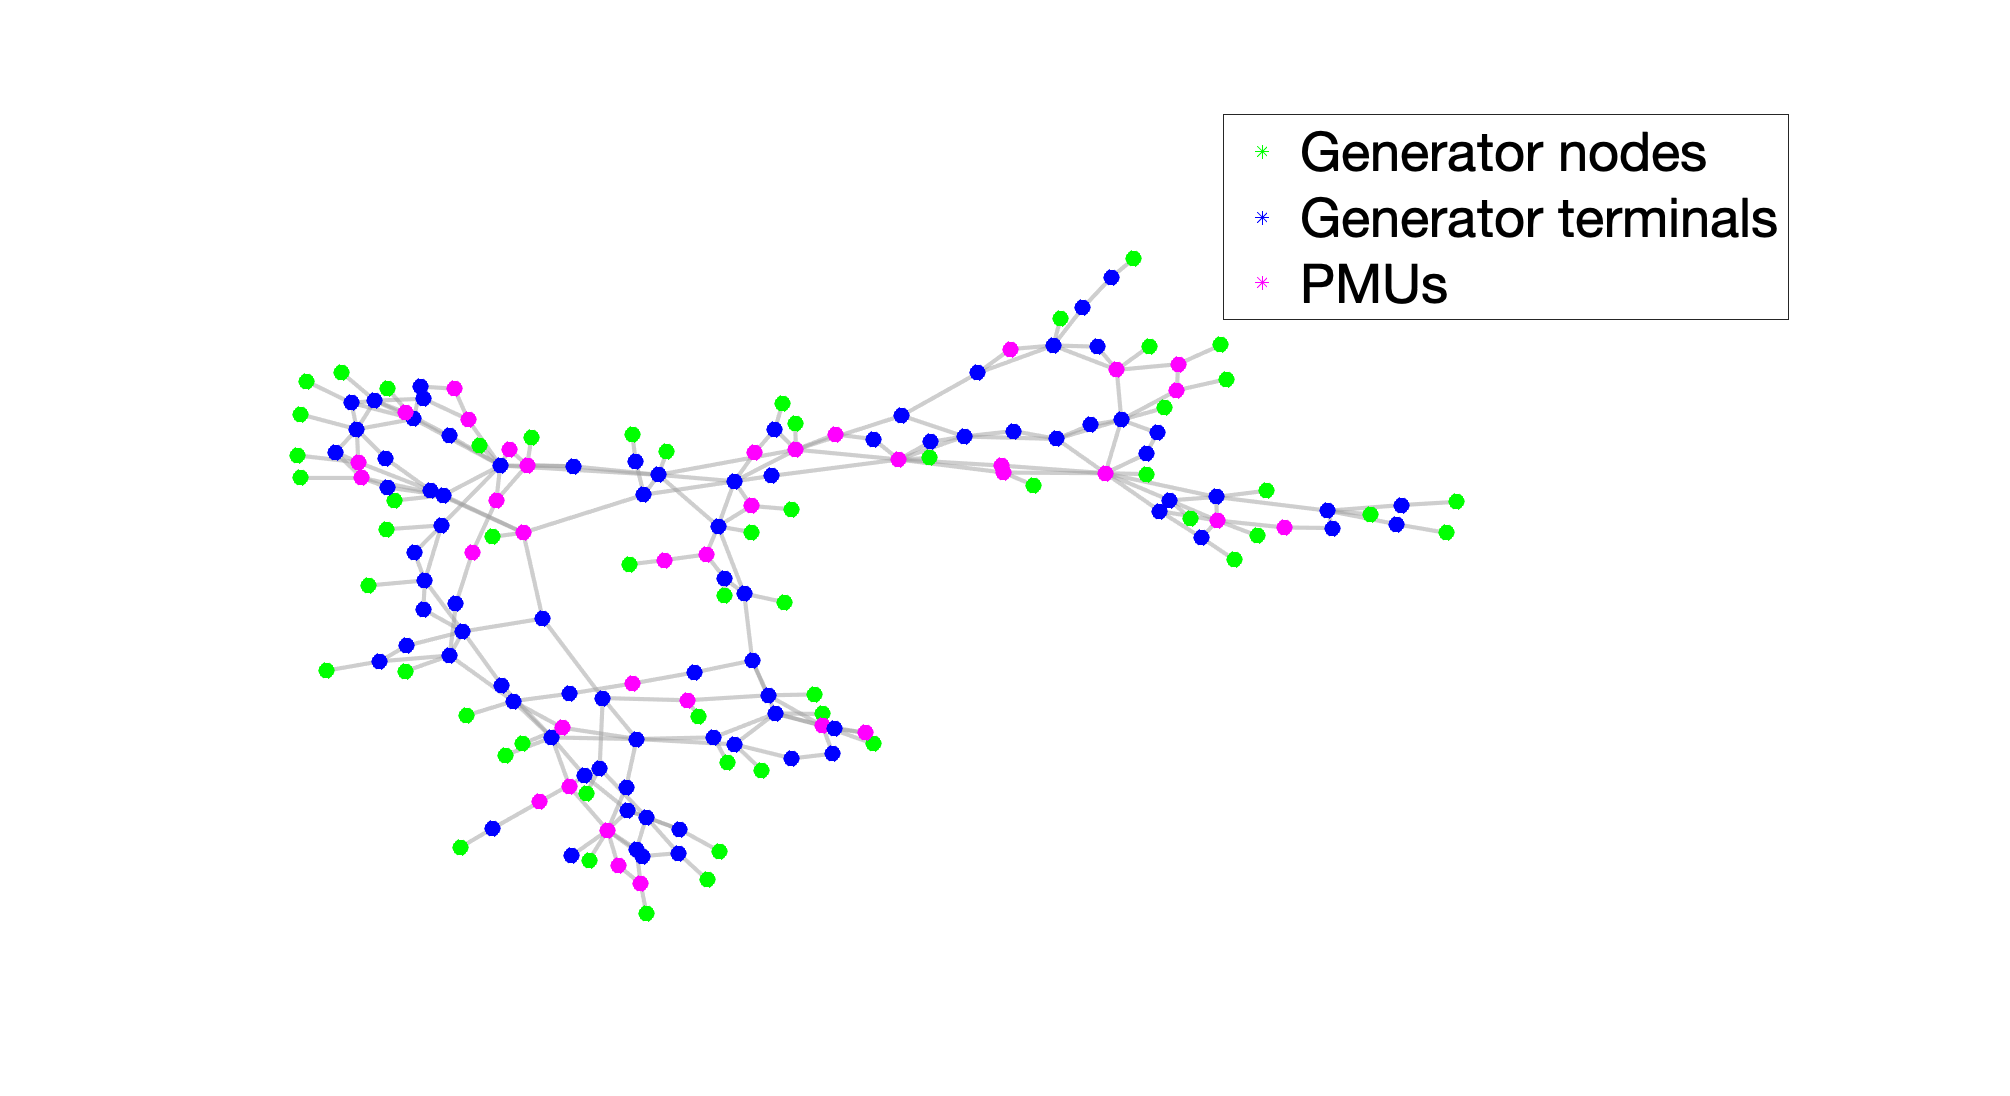
\includegraphics[width=\textheight]{graph-pg}
        \caption{IEEE 118 Power Grid's Dynamic Graph}%
        \label{fig:graph-pg}
      \end{figure}
    \end{column}%
  \end{columns}
\end{slide}

\begin{slide}{Functional Observer}
  \begin{columns}[c]
    \begin{column}{0.48\textwidth}
      \begin{itemize}
        \item \y{} are the measured outputs.
        \item \z{} are the states we wish to estimate.
        \item The observer has a reduced order dynamics system which is
              equivalent to the original one.
        \item Problem 1: how to find a \w{} that correctly estimates \z{}.
        \item Problem 2: how to find the observer's matrices \mN,\mJ,\mH and
              \mE.
      \end{itemize}
    \end{column}%
    \hfill%
    \begin{column}{0.48\textwidth}
      \begin{align}
        \begin{split}
          \dot{x}(t) & = Ax(t) + Bu(t) + Lf(t), \\
          \y         & = Cx(t),                 \\
          \z         & = Fx(t),
        \end{split} \\\nonumber\\
        \begin{split}
          \dw & = \mN\w + \mJ\y + \mH u(t), \\
          \hz & = \w + \mE\y.
        \end{split}
      \end{align}
    \end{column}%
  \end{columns}
\end{slide}

\begin{slide}{Observability}
  \begin{columns}[c]
    \begin{column}{0.48\textwidth}
      \begin{itemize}
        \item All desired states \z{} must be observable from the outputs \y.
        \item The observability of \((A,C,F)\) cannot be greater than that of
              \((A,C)\).
        \item There must be a path from every output \y{} to every output \z{}
              in the dynamics graph.
      \end{itemize}
    \end{column}%
    \hfill%
    \begin{column}{0.48\textwidth}
      \begin{equation}
        rank
        \begin{bmatrix}
          C \\ CA \\ F \\ FA
        \end{bmatrix}
        = rank
        \begin{bmatrix}
          C \\ CA \\ F
        \end{bmatrix}.
      \end{equation}
    \end{column}%
  \end{columns}
\end{slide}

\begin{slide}{Path Finder Algorithm}
  \begin{columns}[c]
    \begin{column}{0.48\textwidth}
      \begin{figure}[ht!]
        \centering \includegraphics[width=0.8\textwidth]{puma560}
        \caption{Puma 560}%
        \label{fig:puma}
      \end{figure}
    \end{column}%
    \hfill%
    \begin{column}{0.48\textwidth}
      \begin{figure}[ht!]
        \centering
        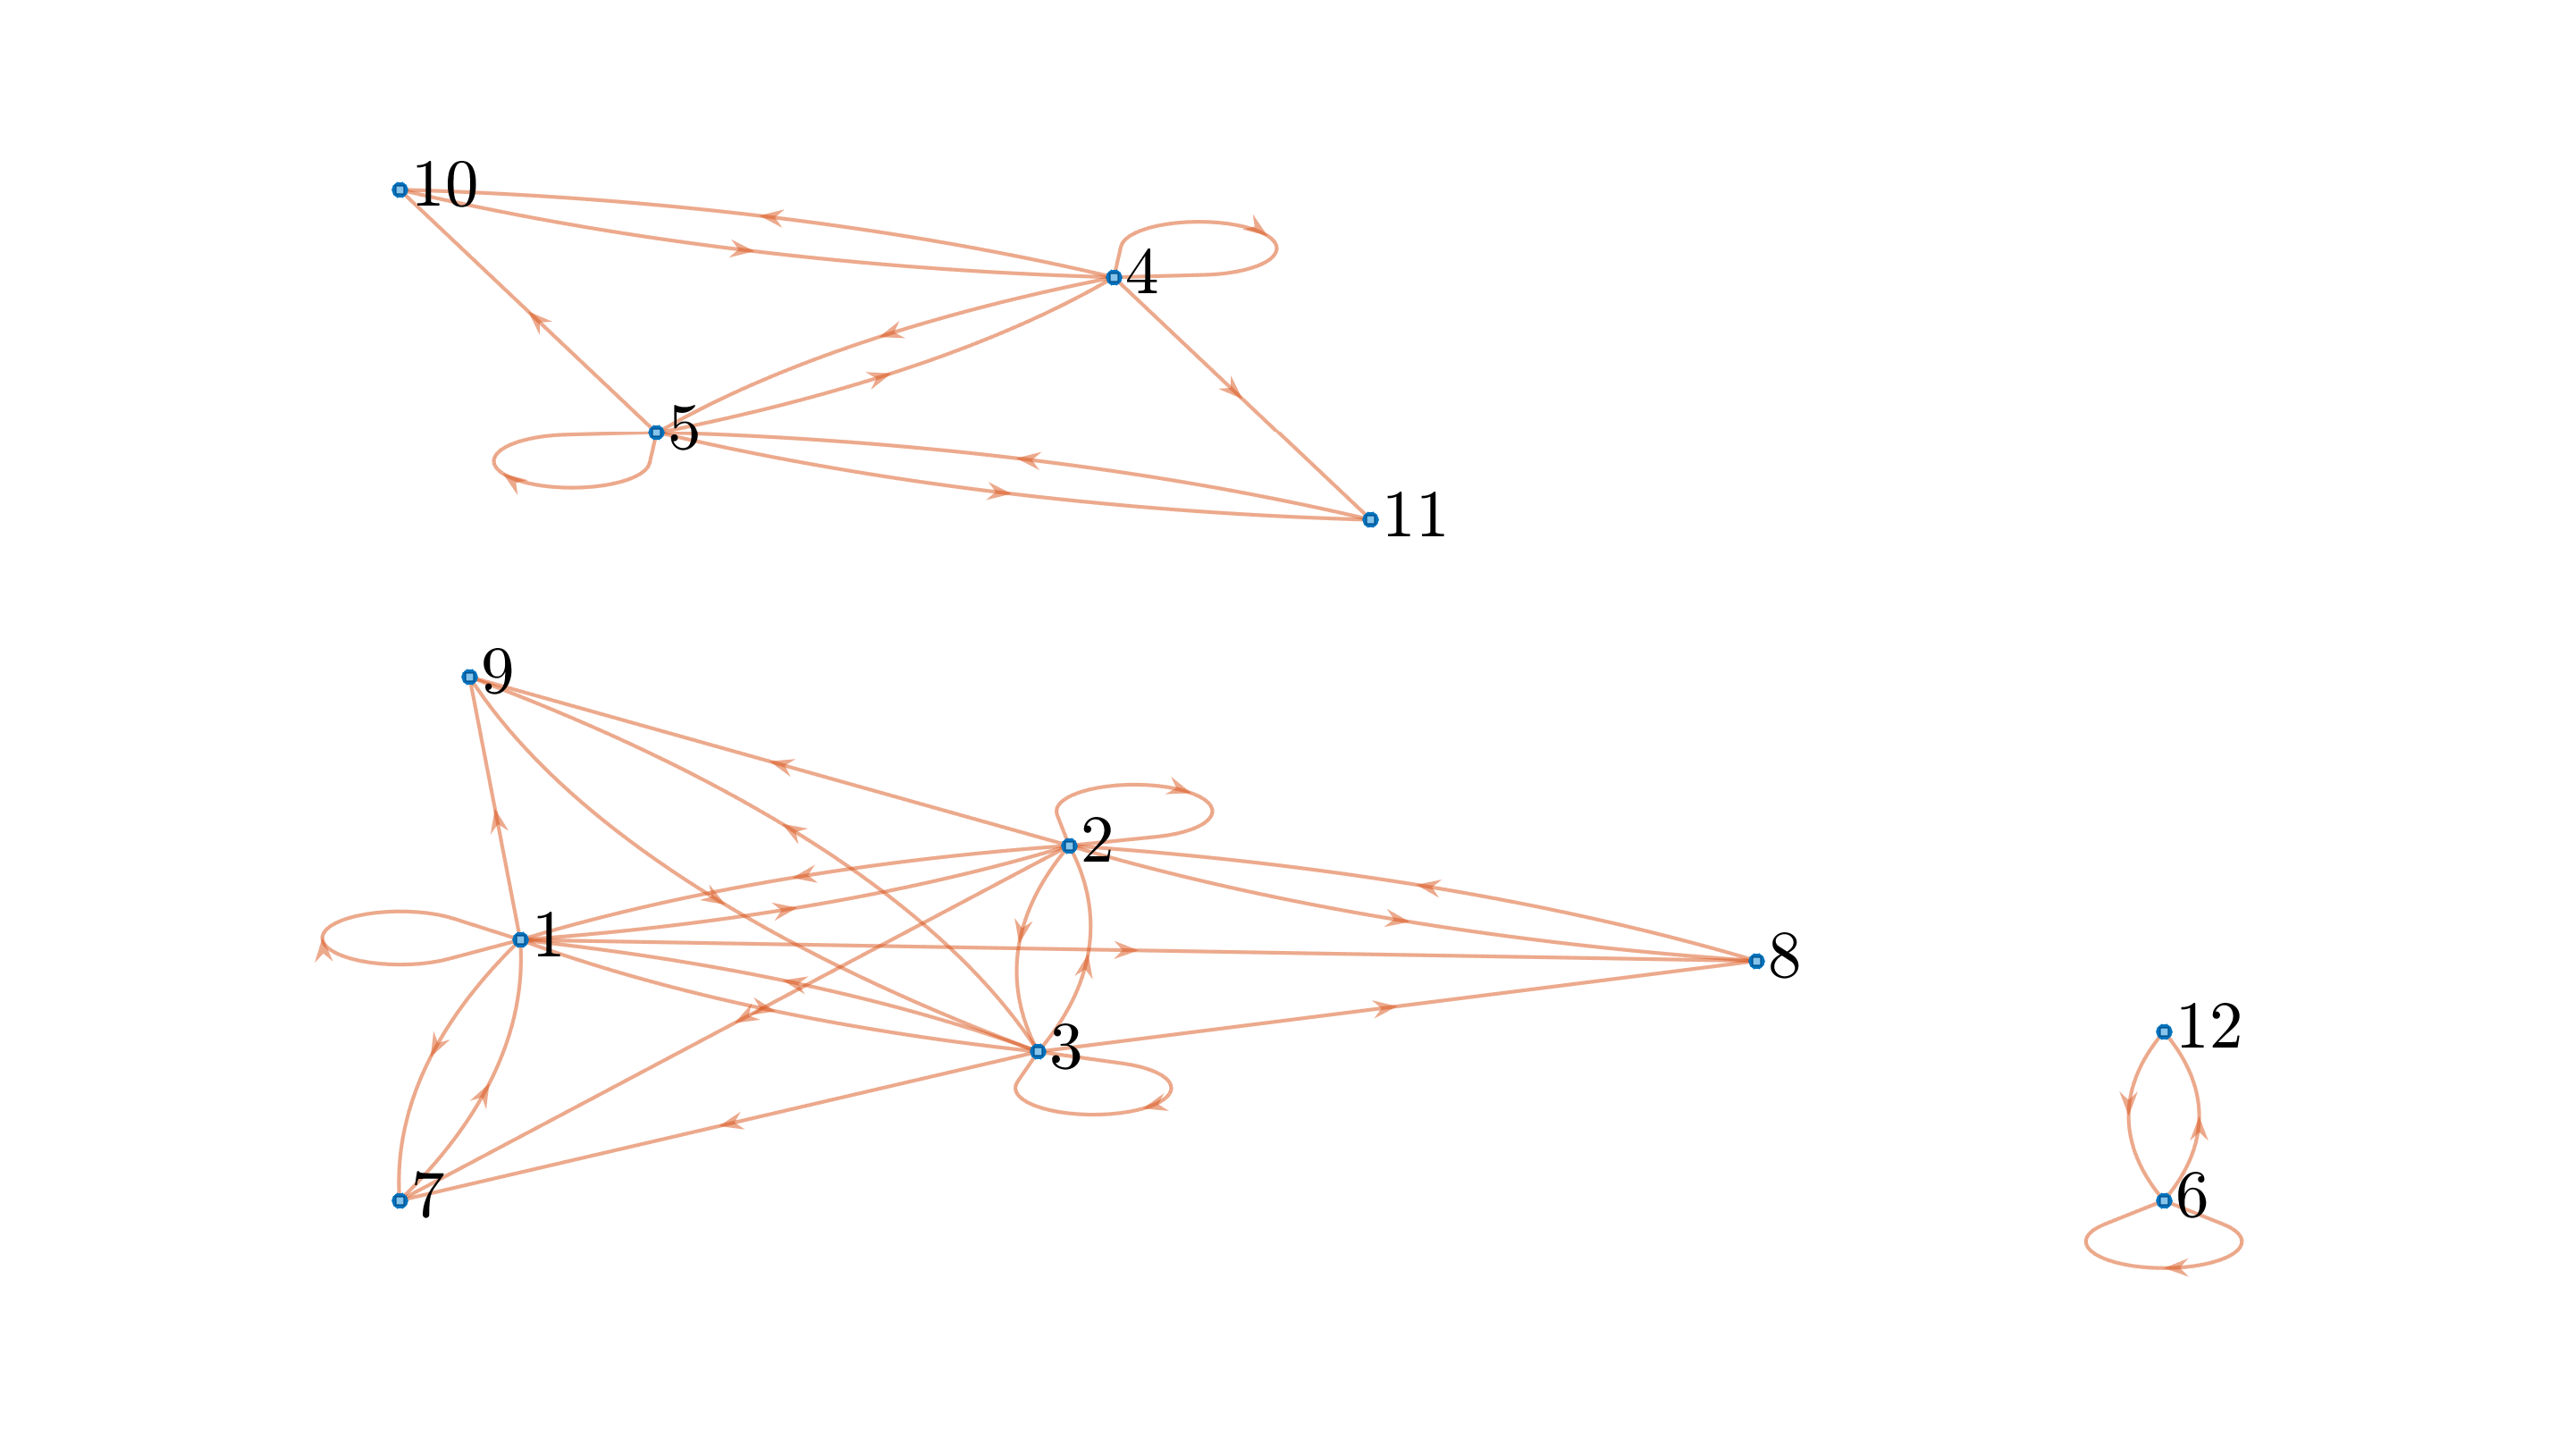
\includegraphics[width=\textwidth]{graph-puma}
        \caption{Puma 560 dynamic's graph representation.}%
        \label{fig:puma-graph}
      \end{figure}
    \end{column}%
  \end{columns}
\end{slide}

% !TeX root = document.tex
% !TeX encoding = UTF-8 Unicode

\subsection{Observer Design}%
\label{subsec:observer-design}

\begin{slide}{Bank of Observers}
  % !TeX root = ../root.tex
% !TeX encoding = UTF-8 Unicode

\begin{figure}[ht!]
  \centering
  \resizebox{\linewidth}{!}{%
    \begin{tikzpicture}[node distance=1cm,block/.style={align=center,draw,shape=rectangle,very thick,minimum height=2em, minimum width=3em},>=stealth]

      \node (ref) []                                      {\(\mathrm{ref}(k)\)};
      \node (C)   [block,right=of ref]                    {Controller};
      \node (G)   [block,right=of C]                      {System};
      \node (y)   [right=2cm of G]                        {\(y(k)\)};
      \node (O)   [block,below=of G]                      {Observer};
      \node (R)   [block,right=of O, below=of y]          {Residual\\Generator};
      \node (r)   [right=of R]                            {\(r(k)\)};
      \node (l)   [below=0.25cm of O.south east]          {one for each sensor};
      \node       [draw,rectangle,dashed,fit=(O) (R) (l)] {};

      \draw [->,thick] (ref) -- (C);
      \draw [->,thick] (C)   -- node (u) [above] {\(u(k)\)} (G);
      \draw [->,thick] (G)   -- (y);
      \draw [->,thick] (u)   |- (O);
      \draw [->,thick] (y)   -- (R);
      \draw [->,thick] (y)   |- ++(0,-0.75) -| (O.north);
      \draw [->,thick] (O)   -- node (w) [above] {\(w(k)\)} (R);
      \draw [->,thick] (R)   -- (r);
    \end{tikzpicture}%
  }
  \caption{Observer's block diagram}%
  \label{fig:schematic}
\end{figure}

\end{slide}

\begin{slide}{Observer Design}
  \begin{columns}[c]
    \begin{column}{0.55\textwidth}
      \begin{equation}
        \begin{aligned}
          \textrm{arg min } & \norm{P}_{2}    \\
          \textrm{s.t. }    & \dot{V} \prec 0 \\
                            & P \succ 0,
        \end{aligned}
      \end{equation}
      %
      where
      %
      \begin{align}
        \dot{V} \equiv & \begin{bmatrix}
                           X        & W  \\
                           W^{\top} & -I
                         \end{bmatrix},                                         \\
        \lambda\in     & \mathbb{R}^{+} \textrm{ is a free constant}, \nonumber \\
        P              & \textrm{ is a semidefinite positve matrix} \nonumber
      \end{align}
      %
      with
      %
      \begin{align}
        \begin{split}
          X = & \hat{A}^{\top}F^{\top}P - \hat{A}^{\top}C^{\top}\hat{E}^{\top} -                 \\
              & \hat{C}^{\top}\hat{K}^{\top} + PF\hat{A} - \hat{E}C\hat{A} - \hat{K}\hat{C} - \lambda{}I,
        \end{split} \\
        W = & \sqrt{\lambda}(PF - \hat{E}C).
      \end{align}
    \end{column}%
    \hfill%
    \begin{column}{0.55\textwidth}
      \begin{align}
        \begin{split}
          \hat{A} & = AF^{+},               \\
          \hat{C} & = CF^{+},               \\
          \hat{E} & = P\mE = PU + \hat{Y}V, \\
          \hat{K} & = PK,                   \\
          \hat{Y} & = PY.
        \end{split} \\\nonumber\\
        \begin{split}
          K   & = P^{-1}\hat{K},  \\
          Y   & = P^{-1}\hat{Y},  \\
          \mE & = U + YV,         \\
          R   & = F - \mE{}C,     \\
          \mN & = (RA - KC)F^{+}, \\
          \mJ & = K + N\mE{},     \\
          \mH & = RB.
        \end{split}
      \end{align}
    \end{column}%
  \end{columns}
\end{slide}

\begin{slide}{Observer Design Development}
  \begin{columns}[c]
    \begin{column}{0.55\textwidth}
      \begin{align}
        \begin{split}
          e & = \hat{z} - z   \\
            & = w + \mE{}y - Fx   \\
            & = w + \mE{}Cx - Fx.
        \end{split} \\
        \begin{split}
          \dot{e} & = \dot{w} + (\mE{}C-F)\dot{x}              \\
                  & = \mN{}w + \mJ{}y + \mH{}u + (\mE{}C-F)(Ax + Bu + Lf)  \\
                  & = \mN{}e + (\mN{}F-\mN{}\mE{}C+\mE{}CA-FA+\mJ{}C)x +           \\
                  & \phantom{=~} (\mH{}+\mE{}CB-FB)u + (\mE{}CL-FL)f.
        \end{split}
      \end{align}
    \end{column}%
    \hfill%
    \begin{column}{0.55\textwidth}
      \begin{align}
        \begin{split}
          \mN{} \textrm{ must be Hurwitz-stable}, &      \\
          \mN{}(F-\mE{}C)-(F-\mE{}C)A+\mJ{}C      & = 0, \\
          \mH{}-(F-\mE{}C)B                       & = 0.
        \end{split} \\\nonumber\\
        \begin{split}
          (F-\mE{}C)L_{i} & = 0,     \\
          (F-\mE{}C)L_{n} & \neq 0.
        \end{split}
      \end{align}
    \end{column}%
  \end{columns}
\end{slide}

\begin{slide}{Observer Design Development}
  \begin{columns}[c]
    \begin{column}{0.55\textwidth}
      \begin{align}
        V             & = e^{\top}Pe,              \\
        \dot{e}       & = \mN{}e-(F-\mE{}C)L_{n}f, \\
        e             & \propto L_{n}f,            \\
        \norm{L_{n}f} & = \lambda{}\norm{e},       \\
        R             & = F-\mE{}C,                \\
        \dot{e}       & = \mN{}e-R\lambda\norm{e}.
      \end{align}
    \end{column}%
    \hfill%
    \begin{column}{0.55\textwidth}
      \begin{align}
        \begin{split}
          \dot{V} & = \dot{e}^{\top}Pe + e^{\top}P\dot{e}                                             \\
                  & = (\mN{}e-\lambda{}R\norm{e})^{\top}Pe + e^{\top}P(\mN{}e-\lambda{}R\norm{e})     \\
                  & = e^{T}(\mN{}^{\top}P + P\mN{})e - 2\lambda\norm{e^{\top}PR}\cdot\norm{e}         \\
                  & \leq e^{T}(\mN{}^{\top}P + P\mN{})e - \lambda(\norm{e^{\top}PR}^{2}+\norm{e}^{2}) \\
                  & = e^{T}(\mN{}^{\top}P + P\mN{} - \lambda{}PRR^{\top}P - \lambda{}I)e.
        \end{split}
      \end{align}
    \end{column}%
  \end{columns}
\end{slide}

\begin{slide}{Observer Design Development}
  \begin{columns}[c]
    \begin{column}{0.55\textwidth}
      \begin{align}
        \begin{split}
          \mN{}(F-\mE{}C) & = RA-\mJ{}C,              \\
          \mN{}F          & = RA-(\mJ{}-\mN{}\mE{})C, \\
          K               & = \mJ{}-\mN{}\mE{},       \\
          \mN{}           & = RAF^{+}-KCF^{+},
        \end{split} \\
        \begin{split}
          (F-\mE{}C)L_{i} & = 0,                                              \\
          \mE{}CL_{i}     & = FL_{i},                                         \\
          \mE{}           & = FL_{i}(CL_{i})^{+} + Y(I-(CL_{i})(CL_{i})^{+}), \\
          U               & = \mE{}CL_{i}L_{i}^{+},                           \\
          V               & = I-L_{i}L_{i}^{+},                               \\
          \mE{}           & = U+YV.
        \end{split}
      \end{align}
    \end{column}%
    \hfill%
    \begin{column}{0.55\textwidth}
      \begin{align}
        \begin{split}
          \dot{V} & = e^{T}((R\hat{A} - \mE{}C\hat{A} - K\hat{C})^{\top}P +                                     \\
                  & P(R\hat{A} - \mE{}C\hat{A} - K\hat{C}) - \lambda{}PRR^{\top}P - \lambda{}I)e.               \\
                  & = \hat{A}^{\top}F^{\top}P - \hat{A}^{\top}C^{\top}\hat{E}^{\top} - \hat{C}^{\top}K^{\top} + \\
                  & PF\hat{A} - \hat{E}C\hat{A} - K\hat{C} - \lambda{}PRR^{\top}P - \lambda{}I.
        \end{split}
      \end{align}
    \end{column}%
  \end{columns}
\end{slide}

\begin{slide}{Residual Generator}
  \begin{columns}[c]
    \begin{column}{0.55\textwidth}
      \begin{align}
        r(t) & = Gw(t) + My(t), \\
        \begin{split}
          M & = (C(1-L_{i}))^{\top},      \\
          G & = -M(I-CF^{+}\mE{})^{-1}CF^{+},
        \end{split}
      \end{align}
    \end{column}%
    \hfill%
    \begin{column}{0.55\textwidth}
      \begin{align}
        \begin{split}
          r & = Gw + My                          \\
            & = Q(y - Cx)                        \\
            & = Q(y - CF^{-1}\hat{z})            \\
            & = Q(y - CF^{-1}(w+\mE{}y))         \\
            & = Q((I-CF^{-1}\mE{})y - CF^{-1}w),
        \end{split} \\
        \begin{split}
          M & = Q(I-CF^{-1}\mE{}), \\
          G & = -QCF^{-1}.
        \end{split}
      \end{align}
    \end{column}%
  \end{columns}
\end{slide}

% !TeX root = document.tex
% !TeX encoding = UTF-8 Unicode

\section{Results}%
\label{sec:results}

\subsection{Robot Arm}%
\label{subsec:robot-arm}

\begin{slide}{Results}
  \begin{columns}[c]
    \begin{column}{0.55\textwidth}
      \begin{figure}[ht!]
        \centering
        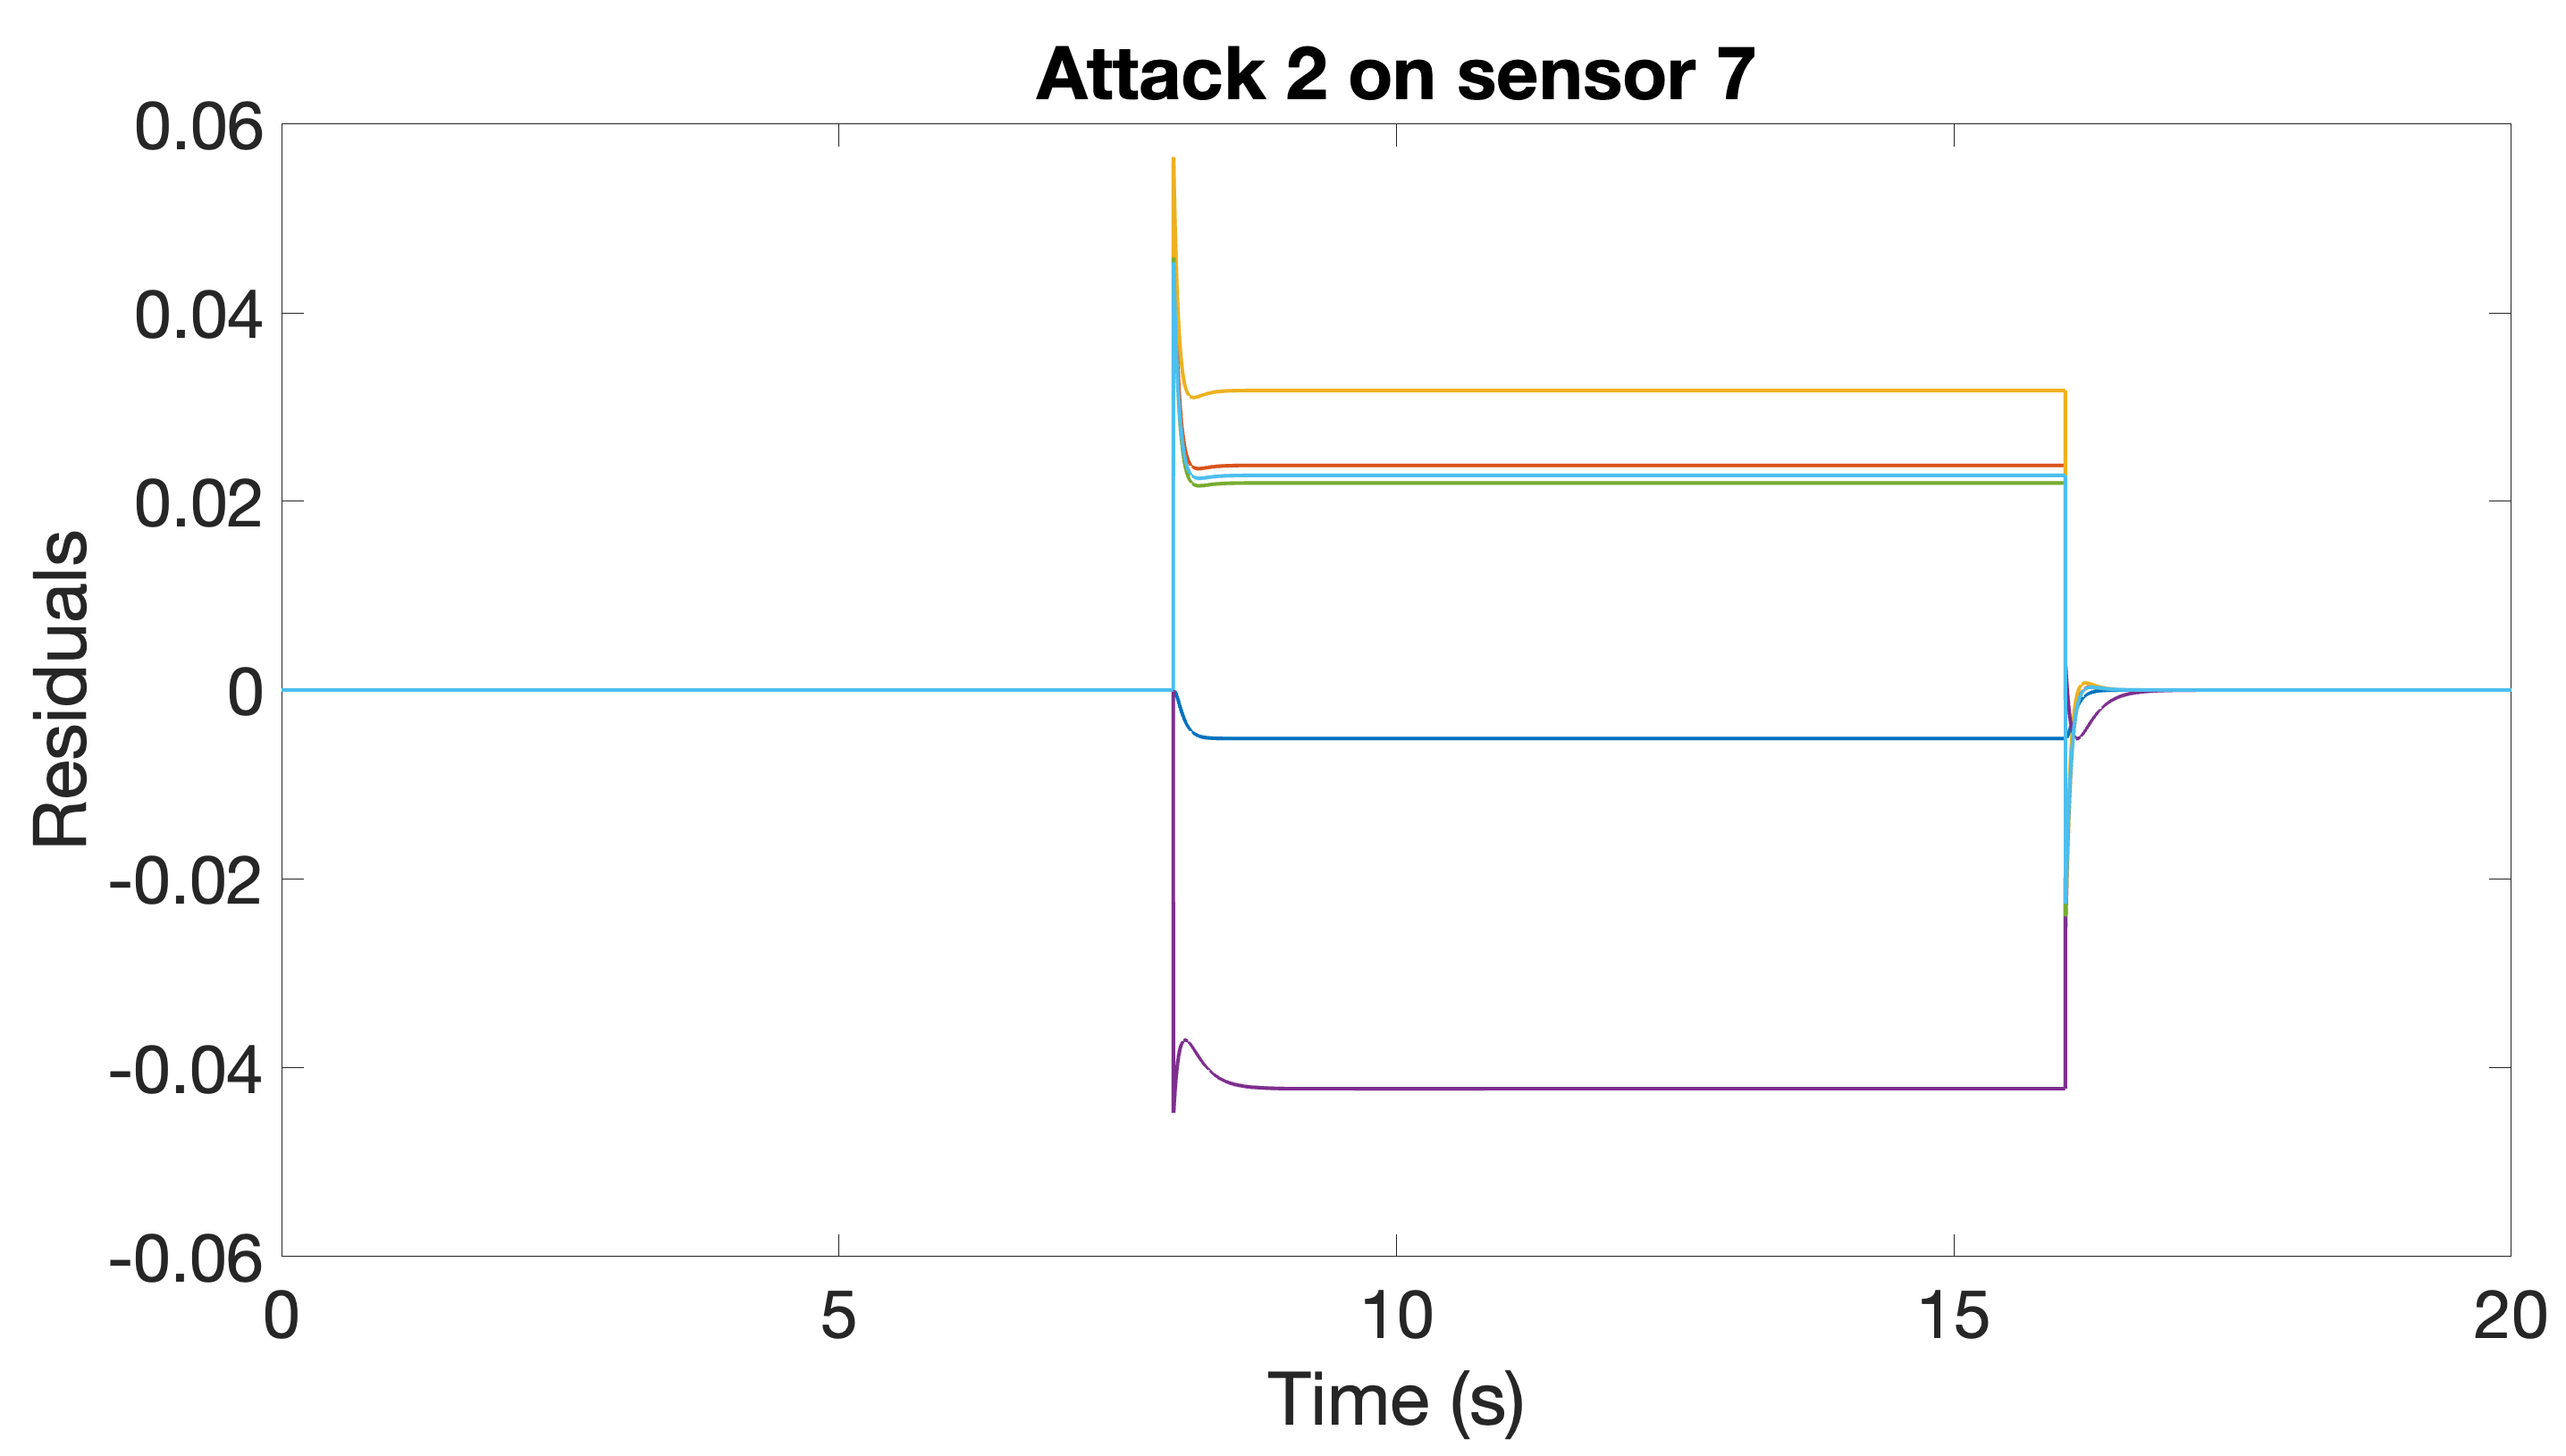
\includegraphics[width=0.9\linewidth]{s7a2}
        \caption{Residuals for attack on sensor 7, with \(\delta=1\).}%
        \label{fig:s7a2}
      \end{figure}
    \end{column}%
    \hfill%
    \begin{column}{0.55\textwidth}
      \begin{figure}[ht!]
        \centering
        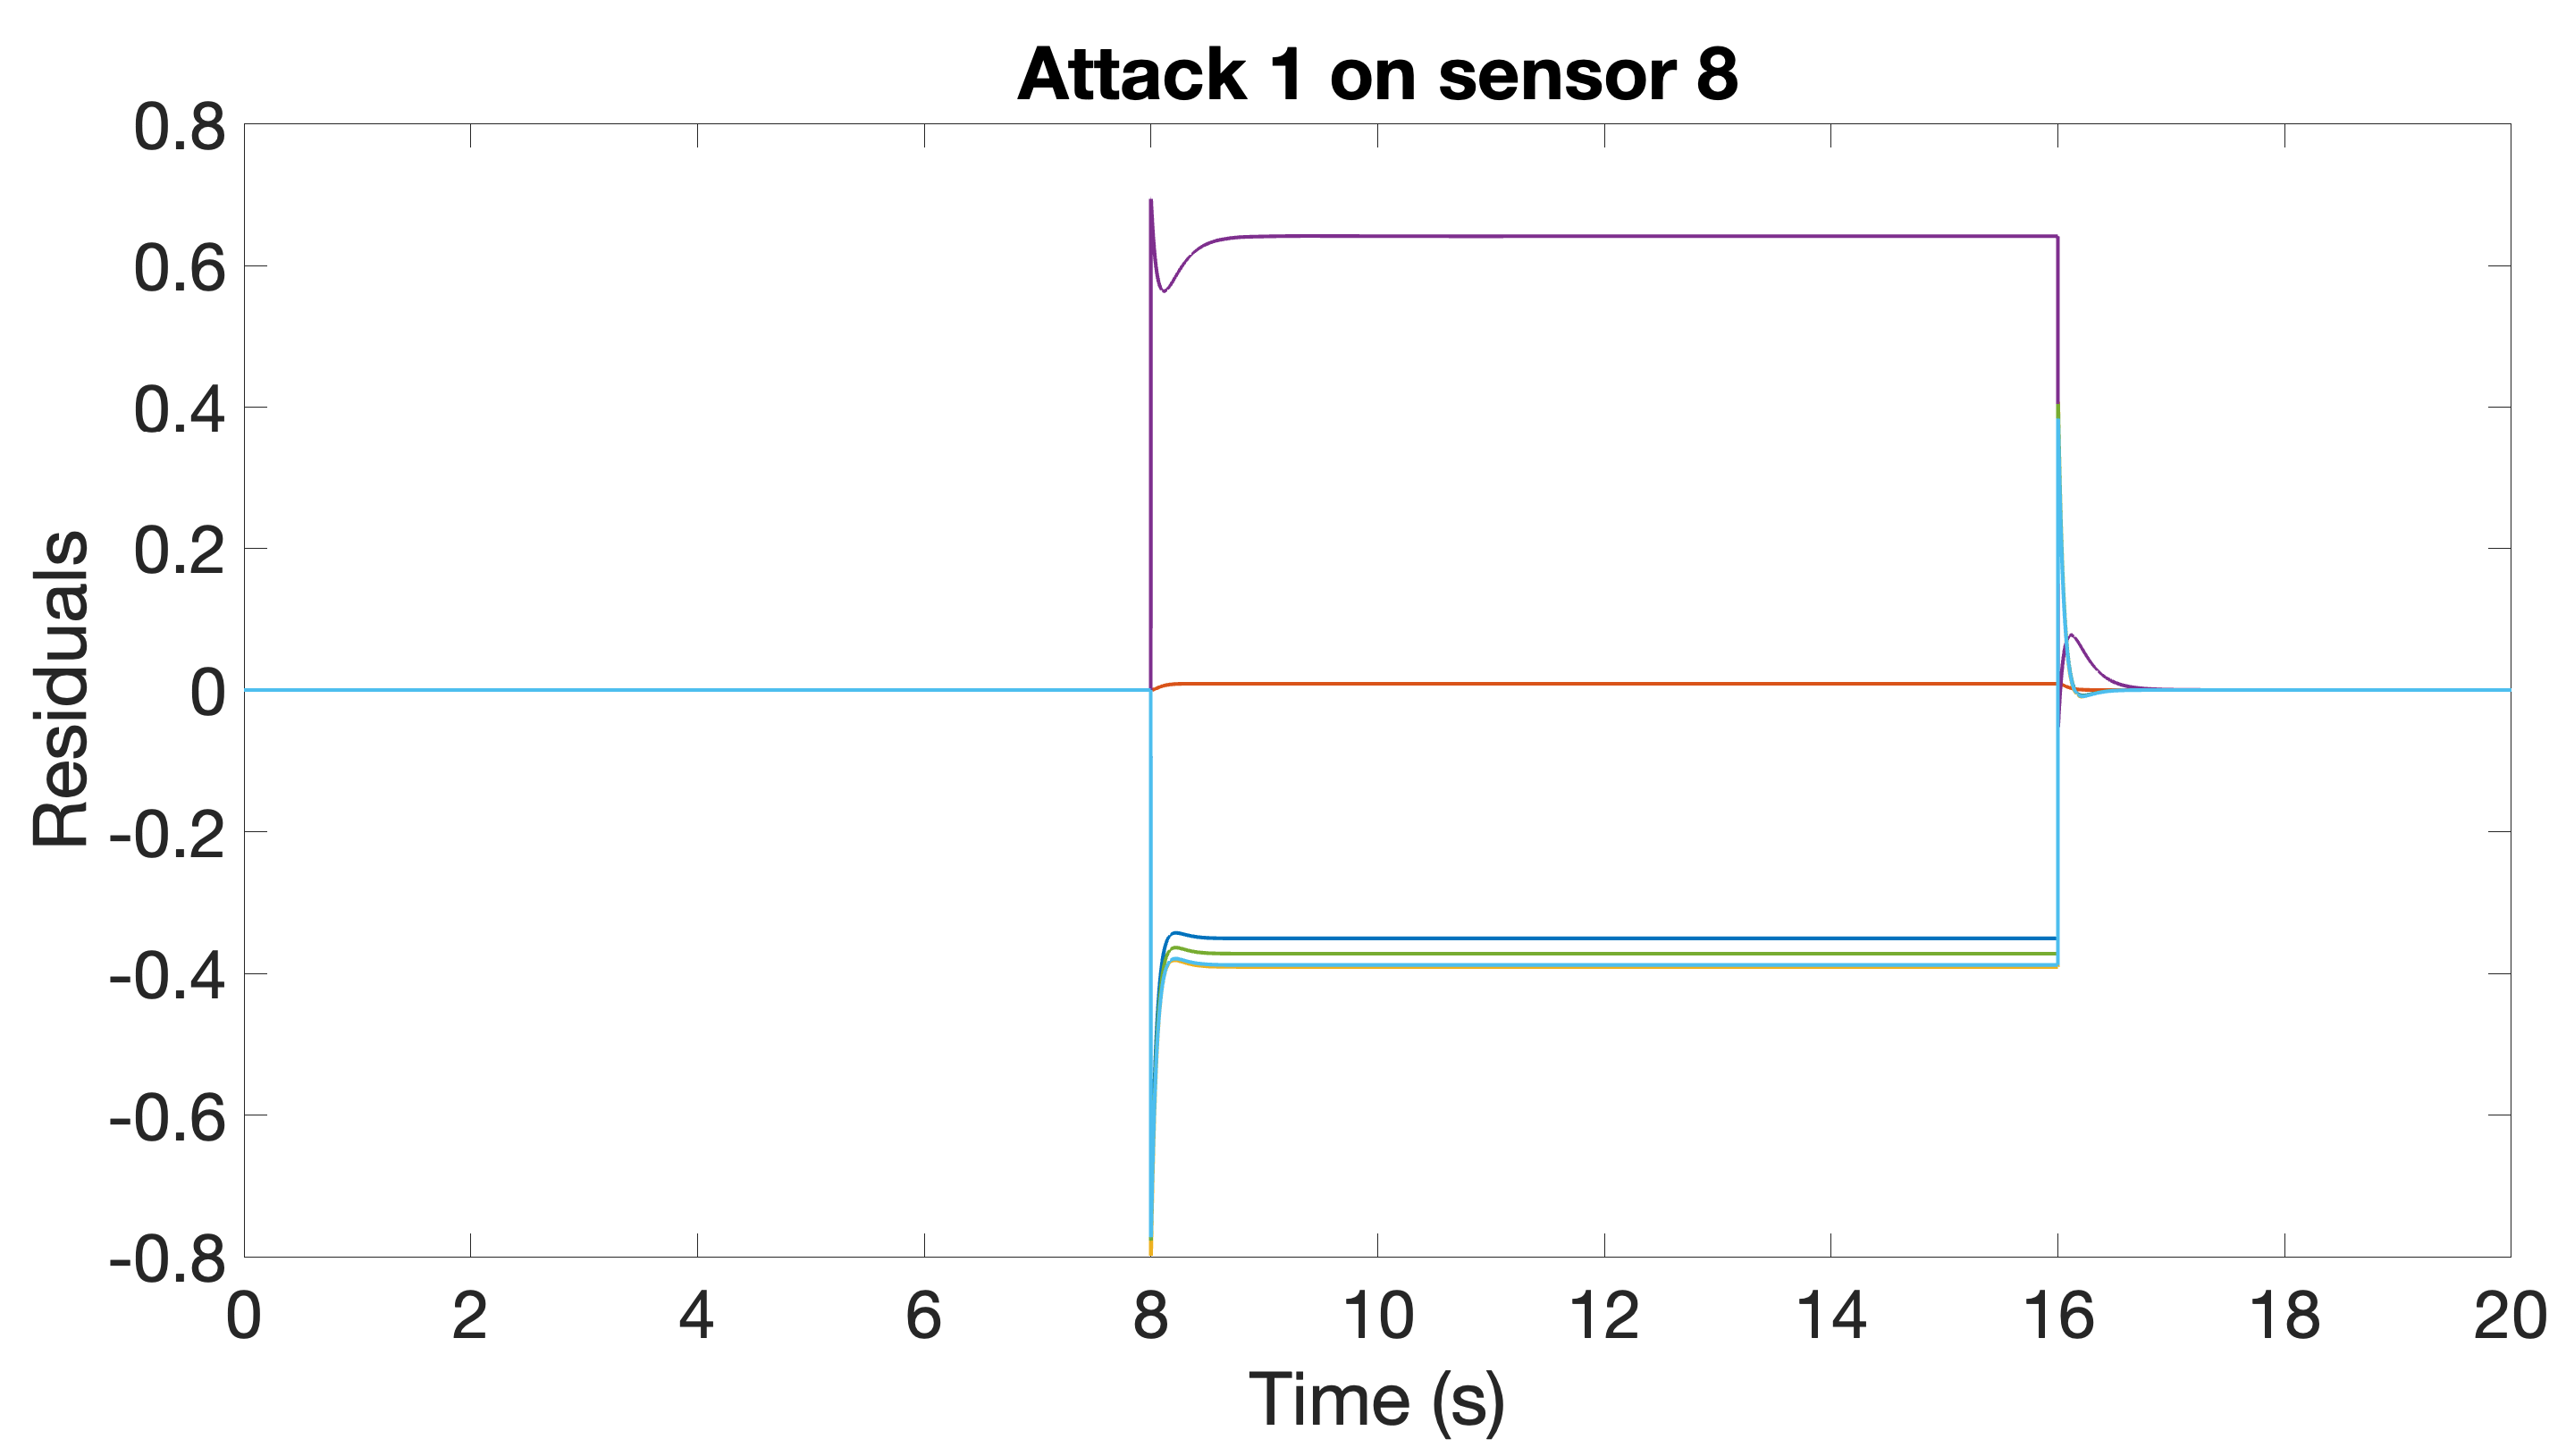
\includegraphics[width=0.9\linewidth]{s8a1}
        \caption{Residuals for attack on sensor 8, copying the values from sensor 9.}%
        \label{fig:s8a1}
      \end{figure}
    \end{column}%
  \end{columns}
\end{slide}

% !TeX root = document.tex
% !TeX encoding = UTF-8 Unicode

\section{Final Considerations}%
\label{sec:conclusion}

\subsection{Final Considerations}%
\label{subsec:conclusion}

\begin{slide}{Final Considerations}
  \begin{itemize}
    \item The formulation is straightforward, optimization based and extendable.
    \item The example was a simple system for didactic reasons, but this kind of
          observer is better suited for large, sparse systems.
  \end{itemize}
\end{slide}

\subsection{Future Works Perspective}%
\label{subsec:future-works}

\begin{slide}{Future Works Perspective}
  \begin{itemize}
    \item Extend to detect Dynamic False Data Injection attacks.
    \item Discrete-time version.
    \item Use with other techniques to detect other types of attacks.
  \end{itemize}
\end{slide}


% !TeX root = document.tex
% !TeX encoding = UTF-8 Unicode

\section{Zero-Dynamics Attack}%
\label{sec:zda}

\subsection{Introduction}%
\label{subsec:ts-introduction}

\begin{slide}{}
  \usebeamercolor{frametitle}
  \vspace*{\fill}
  \begin{center}
    \textcolor{fg}{\Large{Zero-Dynamics Attack}}
  \end{center}
  \vspace*{\fill}
\end{slide}

\begin{slide}{Zero-Dynamics Attack}
  \begin{columns}[c]
    \begin{column}{0.48\textwidth}
      The attacker changes the control signal in a specific direction, taking
      advantage of the system's transmission zeros to change the system's states
      without affecting the system's output.
      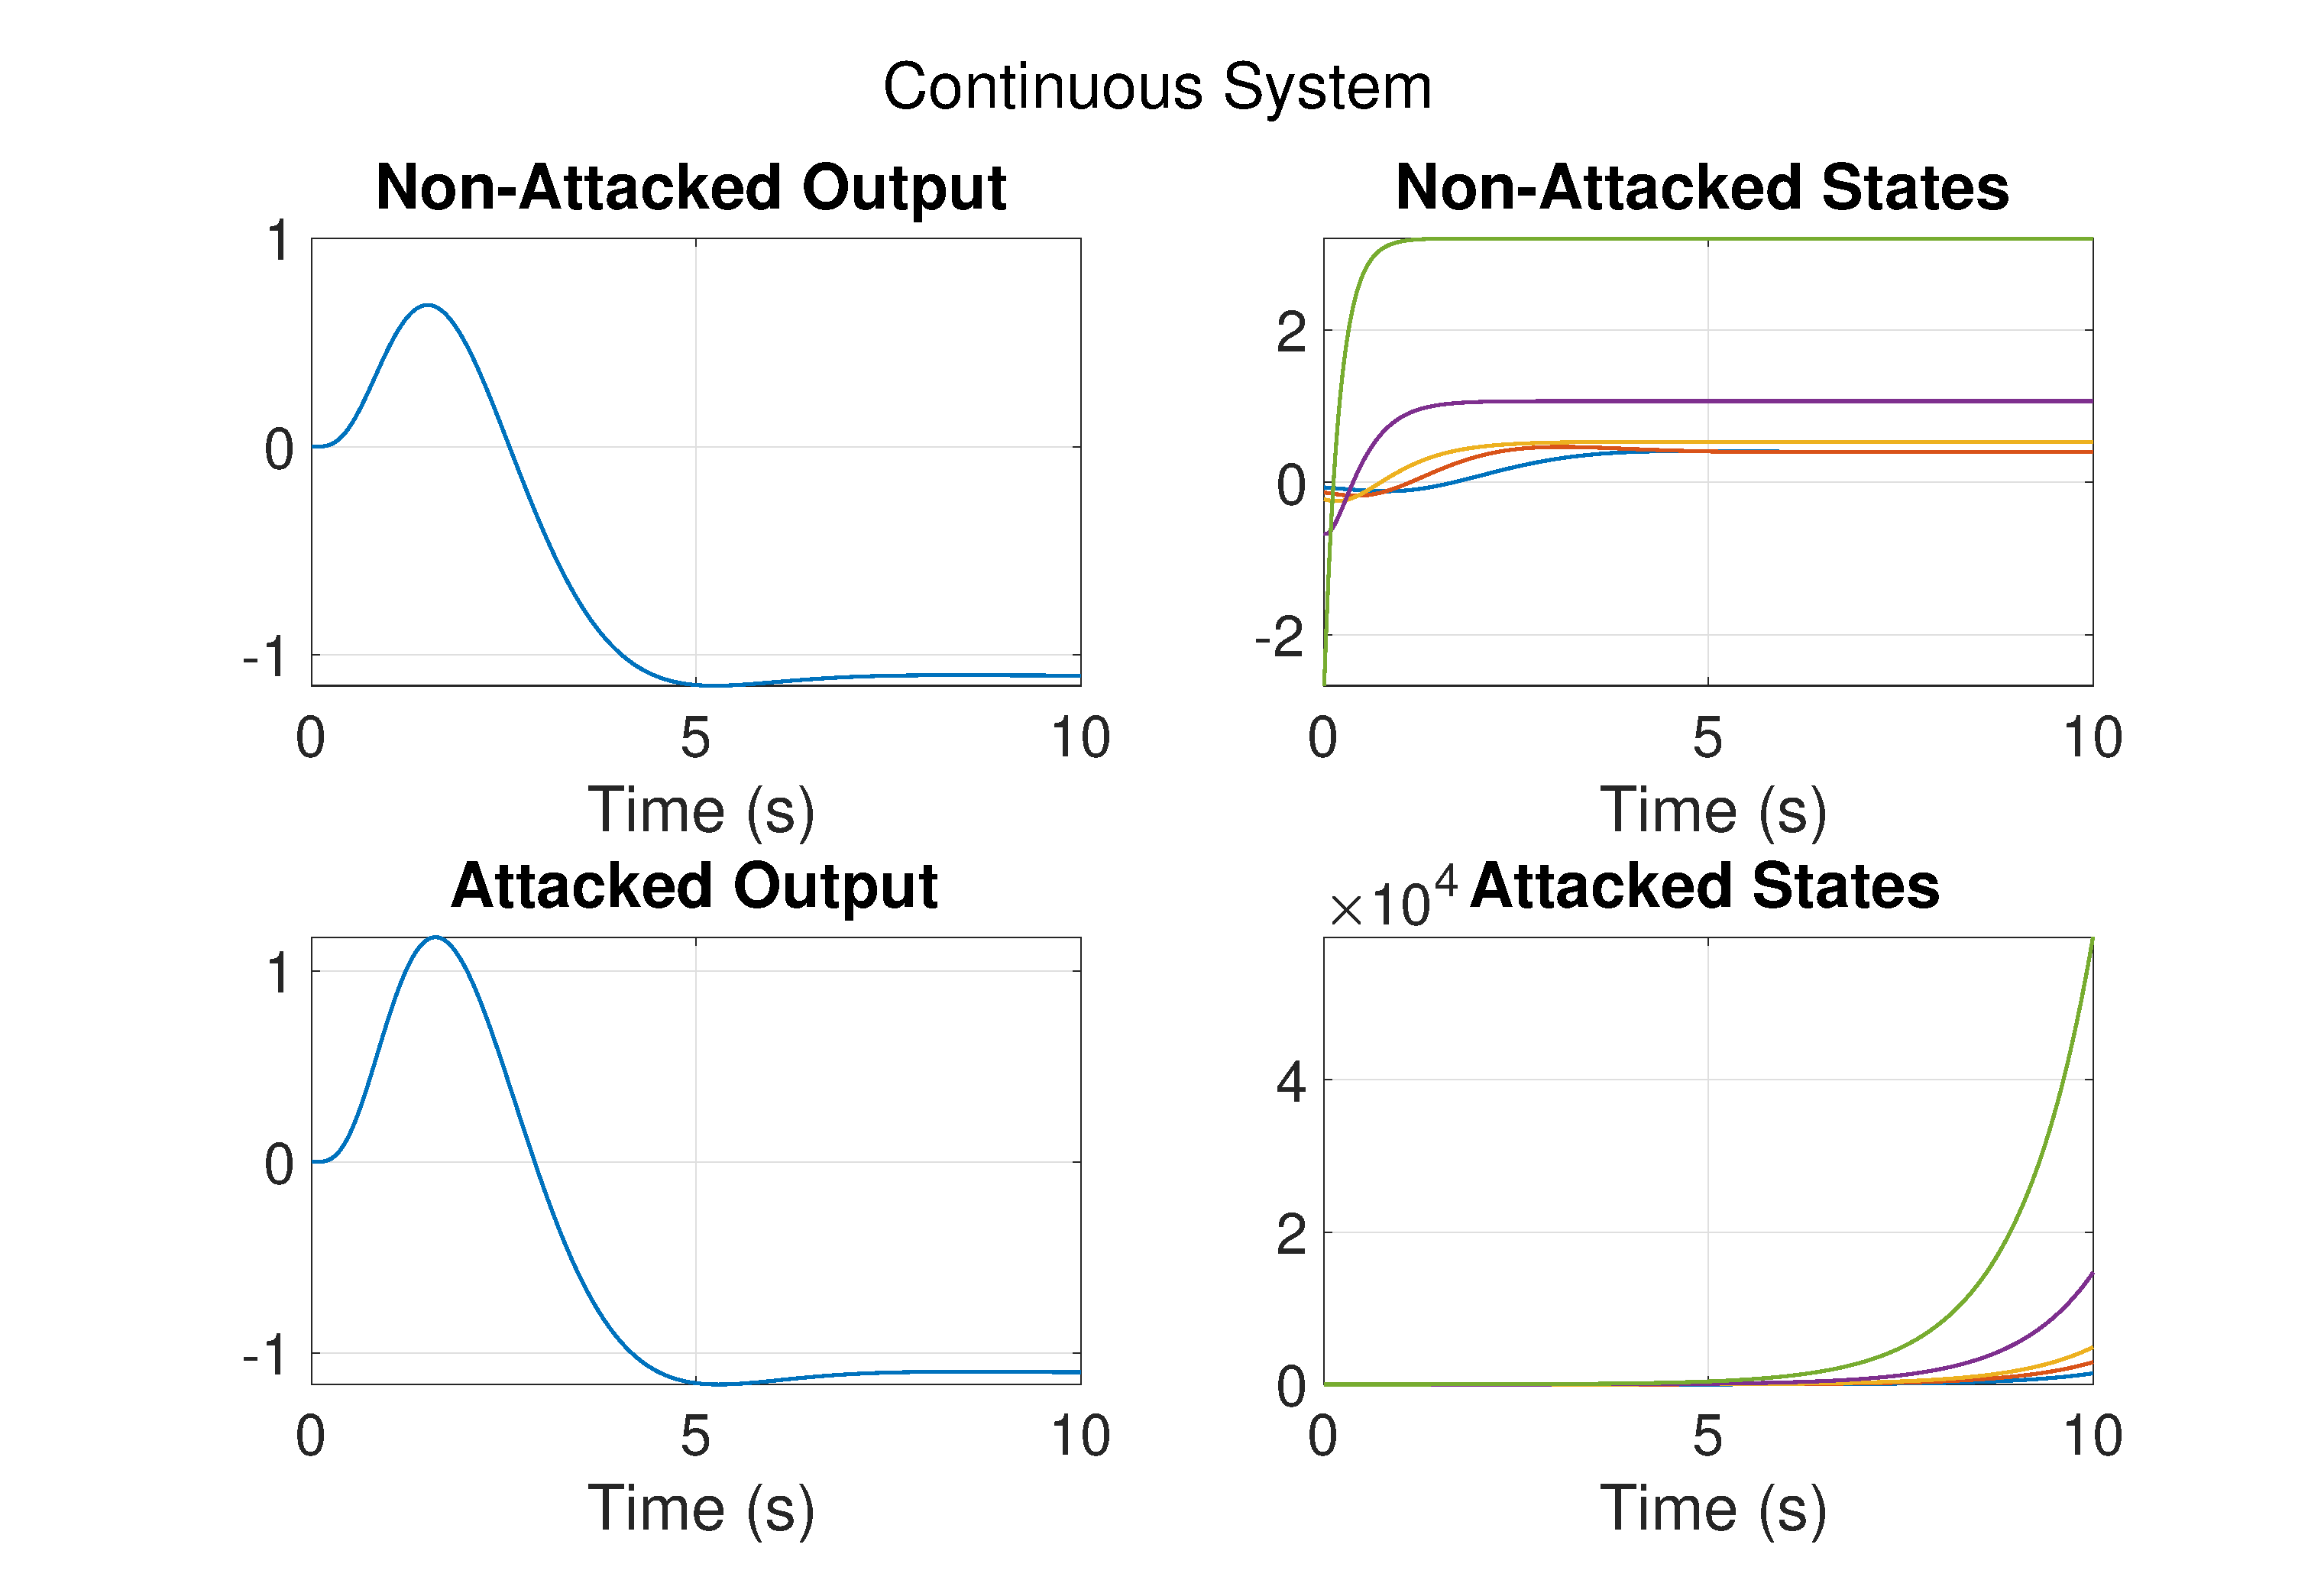
\includegraphics[width=\linewidth]{ct-system}
    \end{column}%
    \hfill%
    \begin{column}{0.48\textwidth}
      \begin{align}
        P(s)          & = \begin{bmatrix}
                            sI-A & -B \\
                            C    & D
                          \end{bmatrix},                                \\
        P(s_{0})z_{0} & = 0.                                            \\
        z_{0}         & = \begin{bmatrix} x_{0} \\ a_{0} \end{bmatrix}, \\
        a(t)          & = a_{0}e^{s_{0}t},                              \\
        \tilde{u}(t)  & =u(t) + a(t).
      \end{align}
    \end{column}%
  \end{columns}
\end{slide}

\begin{slide}{Zero-Dynamics Attack}
  Current detection schemes in the literature:\\~\\
  \begin{itemize}
    \item Generalized Zero-Order Holders
    \item Modified system models
    \item Schemes with multiple observers
  \end{itemize}
\end{slide}

\begin{slide}{Time-Scale Calculus}
  \begin{columns}[c]
    \begin{column}{0.48\textwidth}
      \begin{itemize}
        \item Unifies the continuous- and discrete-time calculi.
        \item Uses the so-called delta-derivative (\(\Delta\)-derivative).
        \item Exists for different time-sets, not only the continuous and
              discrete case.
      \end{itemize}
      \begin{figure}[ht!]
        \centering
        \includegraphics[width=0.6\linewidth]{ts-jump}
        \caption{Time-Scale jump operators. Source: \url{https://shorturl.at/bcJY1}}%
      \end{figure}
    \end{column}%
    \hfill%
    \begin{column}{0.48\textwidth}
      \begin{equation}
        \mathbb{T} = h\mathbb{Z} | \mathbb{R} | \mathbb{T}_{\textrm{iso}}
      \end{equation}
      %
      \begin{align}
        \textrm{forward:~}  & \sigma(t) = \inf\{\tau\in\mathbb{T}|\tau>t\}, \\
        \textrm{backward:~} & \rho(t) = \sup\{\tau\in\mathbb{T}|\tau<t\}.
      \end{align}
      %
      \begin{equation}
        \mu(t) = \sigma(t)-t \leftarrow \textrm{graininess}
      \end{equation}
      %
      \begin{equation}
        f(\sigma(t)) = f(t) + \mu(t)f^{\Delta}(t).
      \end{equation}
    \end{column}%
  \end{columns}
\end{slide}

\begin{slide}{Time-Scale System}
  \begin{columns}[c]
    \begin{column}{0.48\textwidth}
      \begin{itemize}
        \item Allows to evolve the system with arbitrary sampling-times.
        \item Has it own stability criteria based on the Hilger's circle.
      \end{itemize}
    \end{column}%
    \hfill%
    \begin{column}{0.48\textwidth}
      \begin{align}
        x^{\Delta}(t) & = A(\mu(t))x(t) + B(\mu(t))u(t),                      \\
        y(t)          & = Cx(t) + Du(t),                                      \\
        \phantom{1}   & \phantom{1}                                 \nonumber \\
        A(\mu(t))     & = \frac{e^{A\mu(t)}-I}{\mu(t)},                       \\
        B(\mu(t))     & = \int_{0}^{\mu(t)}\frac{e^{(\mu(t)-s)A}}{\mu(t)}Bds.
      \end{align}
    \end{column}%
  \end{columns}
\end{slide}

\begin{slide}{Stability Criteria}
  \begin{columns}[c]
    \begin{column}{0.48\textwidth}
      The system is stable if all of it's poles are within the Hilger's circle,
      defined as a the circle centered at \((-\frac{1}{\mu}, 0)\) and with
      radius \(\frac{1}{\mu}\).

      Note that the circle changes with the sampling-time (\(\mu\)).
    \end{column}%
    \hfill%
    \begin{column}{0.48\textwidth}
      \begin{figure}[ht!]
        \centering
        \resizebox{\linewidth}{!}{%
          \begin{tikzpicture}
            \fill [blue!40!white]           (0, 0) rectangle (1, 2);
            \draw [step=1cm,gray,very thin] (0, 0) grid      (2, 2);
            \node at (1, -0.25) {\(\dot{x}=f(x)\)};

            \fill [blue!40!white]           (3.5, 1) circle (0.5);
            \draw [step=1cm,gray,very thin] (3, 0)   grid   (5, 2);
            \node at (4, -0.25) {\(\Delta{}x=f(x)\)};

            \fill [orange!40!white]         (6.5, 1) circle (0.5);
            \fill [blue!40!white]           (6.6, 1) circle (0.4);
            \fill [green!40!white]          (6.7, 1) circle (0.3);
            \draw [step=1cm,gray,very thin] (6, 0)   grid   (8, 2);
            \node at (7, -0.25) {\(x^{\Delta{}}=f(x)\)};
          \end{tikzpicture}%
        }
        \caption{Different stability regions}%
        \label{fig:stability-regions}
      \end{figure}
    \end{column}%
  \end{columns}
\end{slide}

% !TeX root = document.tex
% !TeX encoding = UTF-8 Unicode

\subsection{Observer Design}%
\label{subsec:ts-observer-design}

\begin{slide}{Observer Design}
  \begin{columns}[c]
    \begin{column}{0.55\textwidth}
      \begin{itemize}
        \item Develop a Lyapunov-based LPV observer.
      \end{itemize}
    \end{column}%
    \hfill%
    \begin{column}{0.55\textwidth}
      \begin{figure}[ht!]
        \centering
        \resizebox{0.6\linewidth}{!}{%
          \begin{tikzpicture}[node distance=1cm,block/.style={align=center,draw,shape=rectangle,very thick,minimum height=2em, minimum width=3em},>=stealth]
            \node (C) [block]                             {Controller};
            \node (G) [block,above=1.5cm of C]            {System};
            \node (H) [block,above=of G]                  {Time-Scale Observer};
            \node (J) [block,above=of H]                  {Residual Generator};
            \node (u) [above left=0.5cm and 1cm of C]     {\(u(t)\)};
            \node (y) [above right=0.5cm and 1cm of C]    {\(y(t)\)};
            \node (r) [right=0.5cm of J]                  {\(r(t)\)};
            \node     [draw,rectangle,dashed,fit=(u) (y)] {Network};

            \draw [->,thick] (C) -| (u) |- (G);
            \draw [->,thick] (G) -| (y) |- (C);
            \draw [->,thick] (u) |- (H);
            \draw [->,thick] (y) |- (H);
            \draw [->,thick] (H) -- (J) -- (r);
          \end{tikzpicture}%
        }
        \caption{Observer's block diagram}%
        \label{fig:ts-schematic}
      \end{figure}
    \end{column}%
  \end{columns}
\end{slide}

\begin{slide}{Observer Design Development}
  \begin{columns}[c]
    \begin{column}{0.55\textwidth}
      \begin{align}
        x^{\Delta} & = Ax + Bu, \\
        y          & = Cx,
      \end{align}
      %
      \begin{gather}
        V = x\tr{}Px
      \end{gather}
      %
      \begin{gather}
        x(\sigma(t)) = x(t) + \mu(t)x^{\Delta}(t).
      \end{gather}
      %
      \begin{gather}
        PA + A\tr{}P + \mu{}A\tr{}PA \prec{} 0 \\
        P \succ{} 0
      \end{gather}
    \end{column}%
    \hfill%
    \begin{column}{0.55\textwidth}
      \begin{gather}
        \begin{bmatrix}
          M     & (PA - ZC)  \\
          \star & -\mu^{-1}P
        \end{bmatrix} \prec{} 0,  \\
        M = PA + A\tr{}P - ZC - C\tr{}Z\tr{}.
      \end{gather}
      %
      \begin{equation}
        Z = PL.
      \end{equation}
      %
      \begin{equation}
        x^{\Delta} = Ax + Bu -L(y - Cx).
      \end{equation}
    \end{column}%
  \end{columns}
\end{slide}

\begin{slide}{Observer Design Development}
  \begin{columns}[c]
    \begin{column}{0.55\textwidth}
      An LPV observer for a time-scale system of the form
      %
      \begin{align}
        \hat{x}^{\Delta} & = A(\mu)\hat{x} + B(\mu)u - L(\mu)(y - C\hat{x}),                                                                                                            \\
        L(\mu)           & = \sum_{i=0}^{3}\alpha_{i}(\mu)L_{i},                                                                                                                        \\
        \alpha_{0}(\mu)  & = \textcolor{frenchblue}{\frac{\bar{\mu}^{-1}-\mu^{-1}}{\bar{\mu}^{-1}-\ubar{\mu}^{-1}}}  \textcolor{flame}{\frac{\bar{\mu}-\mu}{\bar{\mu}-\ubar{\mu}}},  \\
        \alpha_{1}(\mu)  & = \textcolor{frenchblue}{\frac{\mu^{-1}-\ubar{\mu}^{-1}}{\bar{\mu}^{-1}-\ubar{\mu}^{-1}}} \textcolor{flame}{\frac{\bar{\mu}-\mu}{\bar{\mu}-\ubar{\mu}}},  \\
        \alpha_{2}(\mu)  & = \textcolor{frenchblue}{\frac{\bar{\mu}^{-1}-\mu^{-1}}{\bar{\mu}^{-1}-\ubar{\mu}^{-1}}}  \textcolor{flame}{\frac{\mu-\ubar{\mu}}{\bar{\mu}-\ubar{\mu}}}, \\
        \alpha_{3}(\mu)  & = \textcolor{frenchblue}{\frac{\mu^{-1}-\ubar{\mu}^{-1}}{\bar{\mu}^{-1}-\ubar{\mu}^{-1}}} \textcolor{flame}{\frac{\mu-\ubar{\mu}}{\bar{\mu}-\ubar{\mu}}},
      \end{align}
    \end{column}%
    \hfill%
    \begin{column}{0.55\textwidth}
      \begin{align}
                 & \begin{bmatrix}
                     M(\cubar{\mu},0) & PA(\cubar{\mu}) - Z_{0}C \\
                     \star            & -\frac{1}{\cubar{\mu}}P
                   \end{bmatrix} \prec{} 0,  \\
                 & \begin{bmatrix}
                     M(\cbar{\mu},1) & PA(\cbar{\mu}) - Z_{1}C \\
                     \star           & -\frac{1}{\cubar{\mu}}P
                   \end{bmatrix} \prec{} 0,    \\
                 & \begin{bmatrix}
                     M(\cubar{\mu},2) & PA(\cubar{\mu}) - Z_{2}C \\
                     \star            & -\frac{1}{\cbar{\mu}}P
                   \end{bmatrix} \prec{} 0, \\
                 & \begin{bmatrix}
                     M(\cbar{\mu},3) & PA(\cbar{\mu}) - Z_{3}C \\
                     \star           & -\frac{1}{\cbar{\mu}}P
                   \end{bmatrix} \prec{} 0,   \\
        M(\mu,i) & = PA(\mu) + A(\mu)\tr{}P - Z_{i}C - C\tr{}Z_{i}\tr,     \\
        L_{i}    & = P^{-1}Z_{i}.
      \end{align}
    \end{column}%
  \end{columns}
\end{slide}

% !TeX root = document.tex
% !TeX encoding = UTF-8 Unicode

\subsection{Results}%
\label{subsec:ts-results}

\begin{slide}{Results}
  \begin{columns}[c]
    \begin{column}{0.55\textwidth}
      \begin{figure}[ht!]
        \centering
        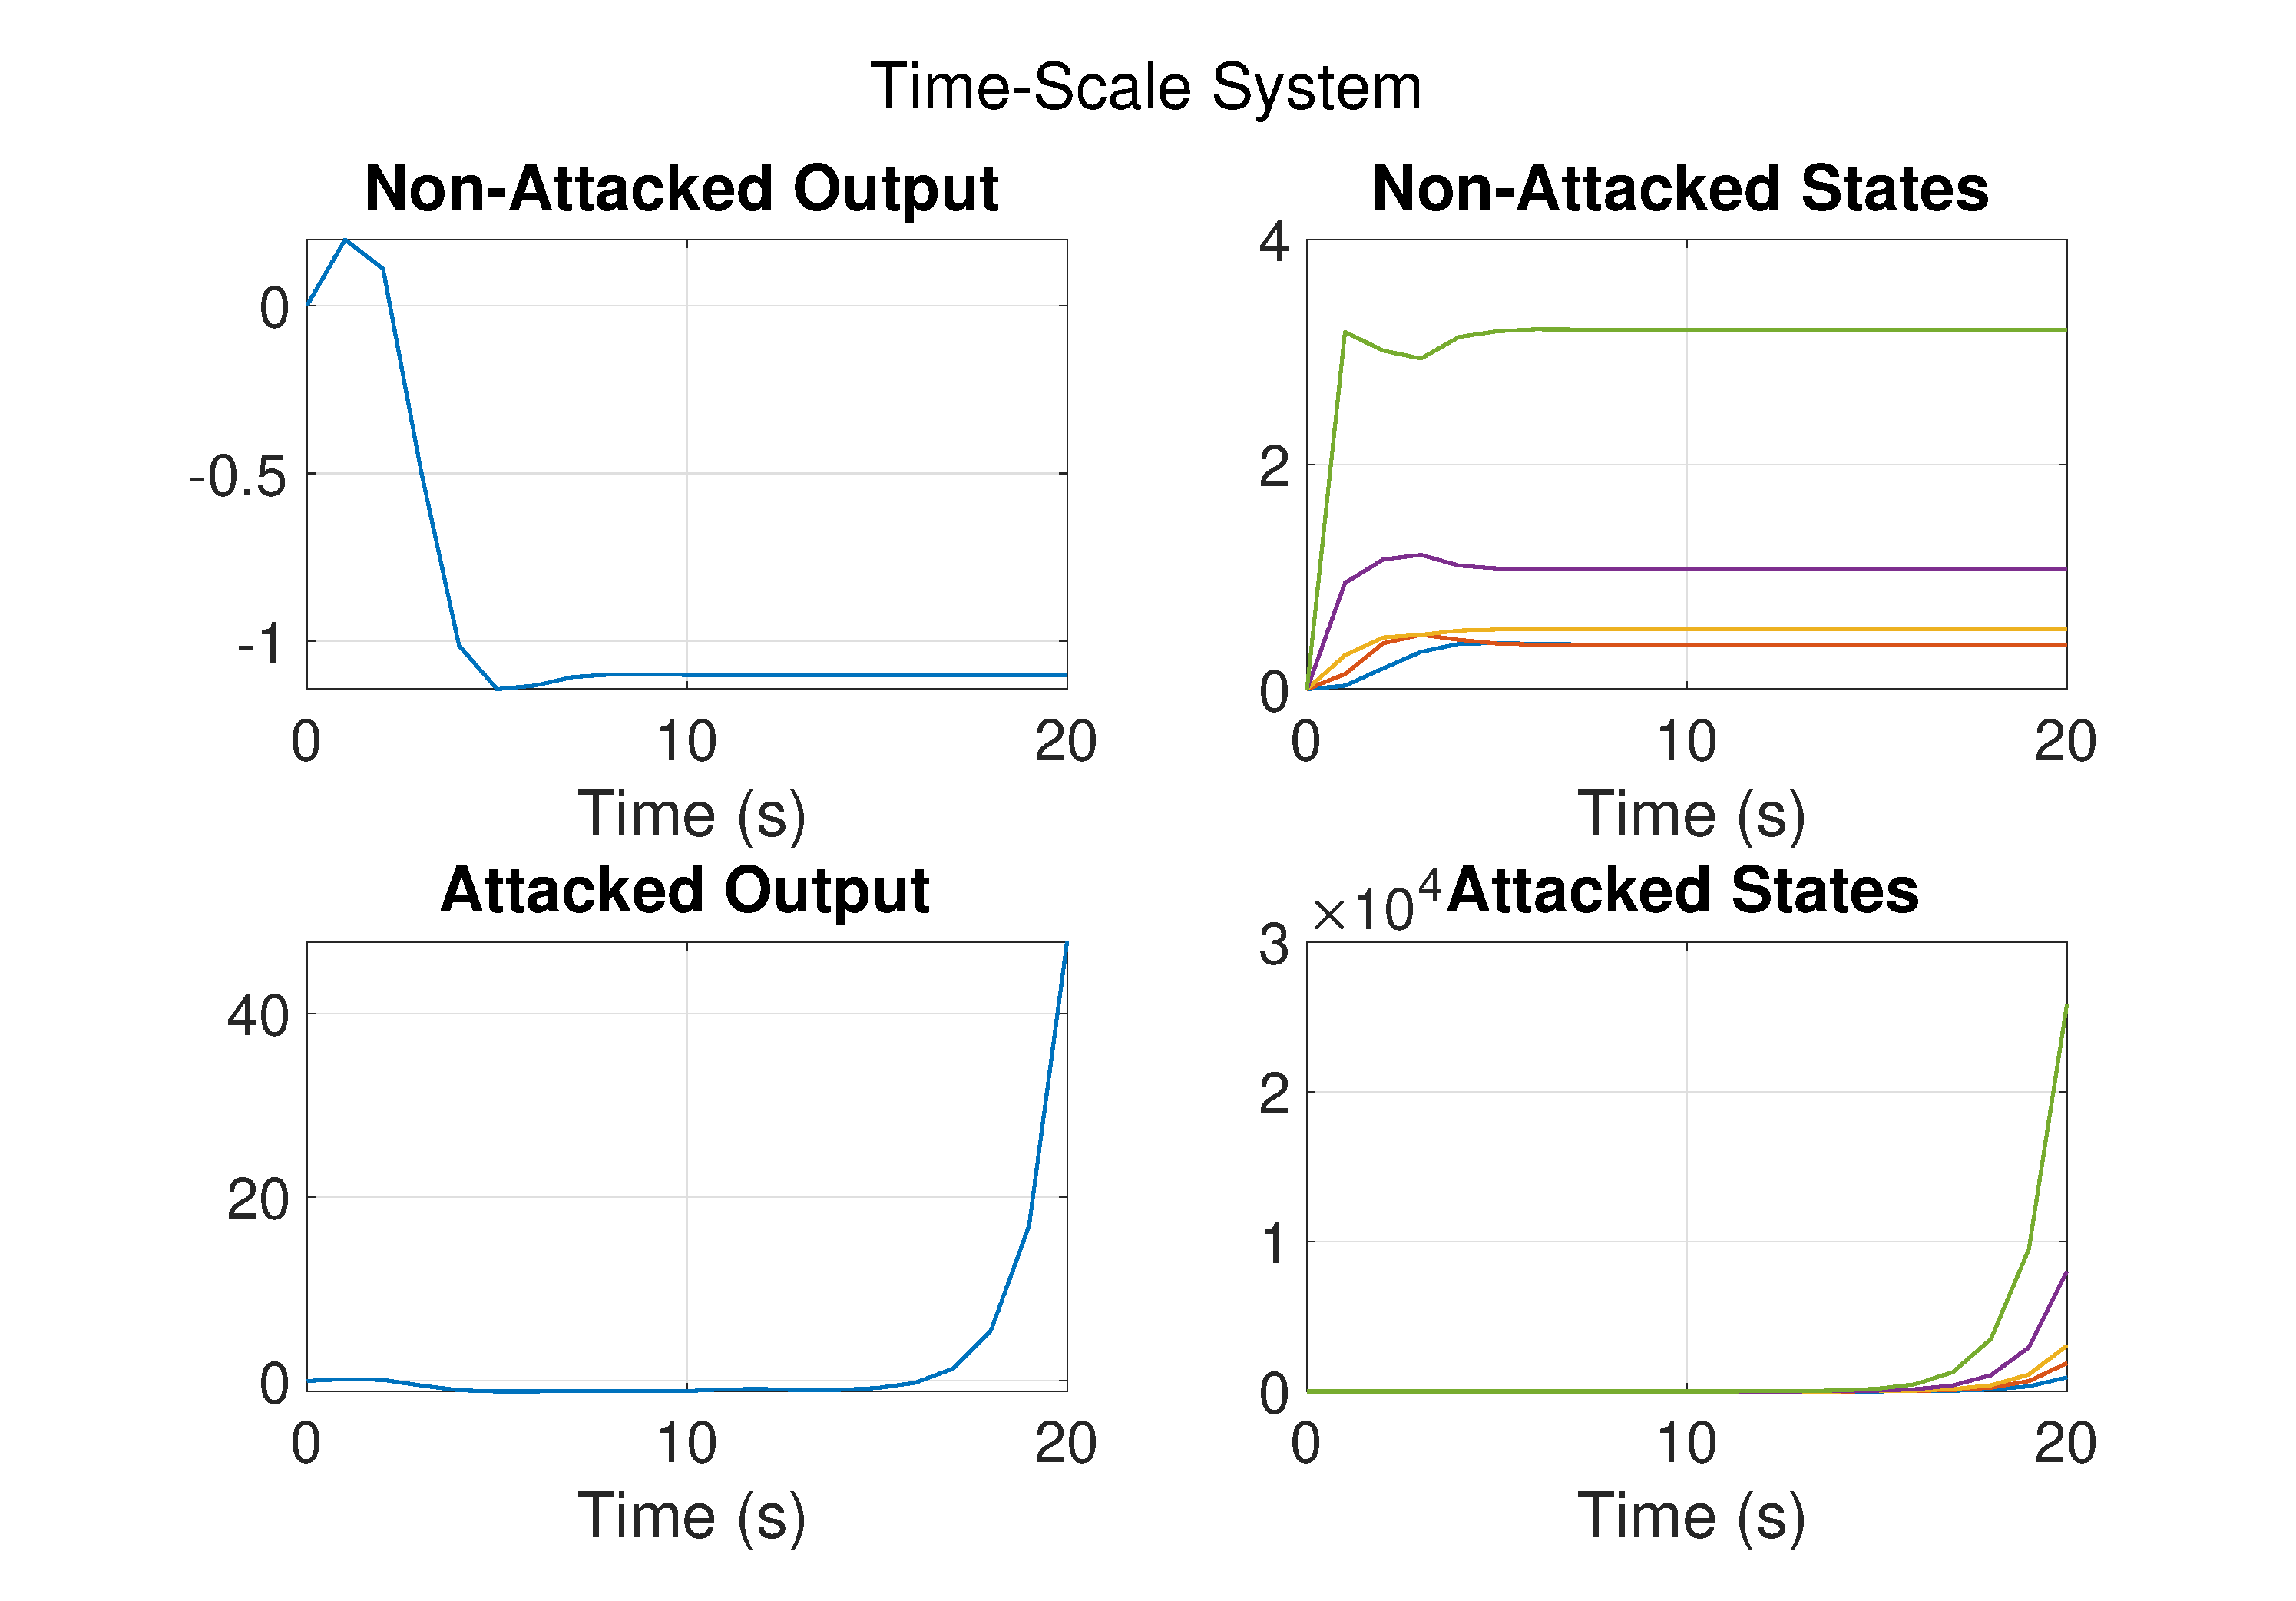
\includegraphics[width=\linewidth]{ts-system}
        \caption{Time-scale system's observer with \(\mu=\SI{1}{\second}\).}%
        \label{fig:ct-system}
      \end{figure}
    \end{column}%
    \hfill%
    \begin{column}{0.55\textwidth}
      \begin{figure}[ht!]
        \centering
        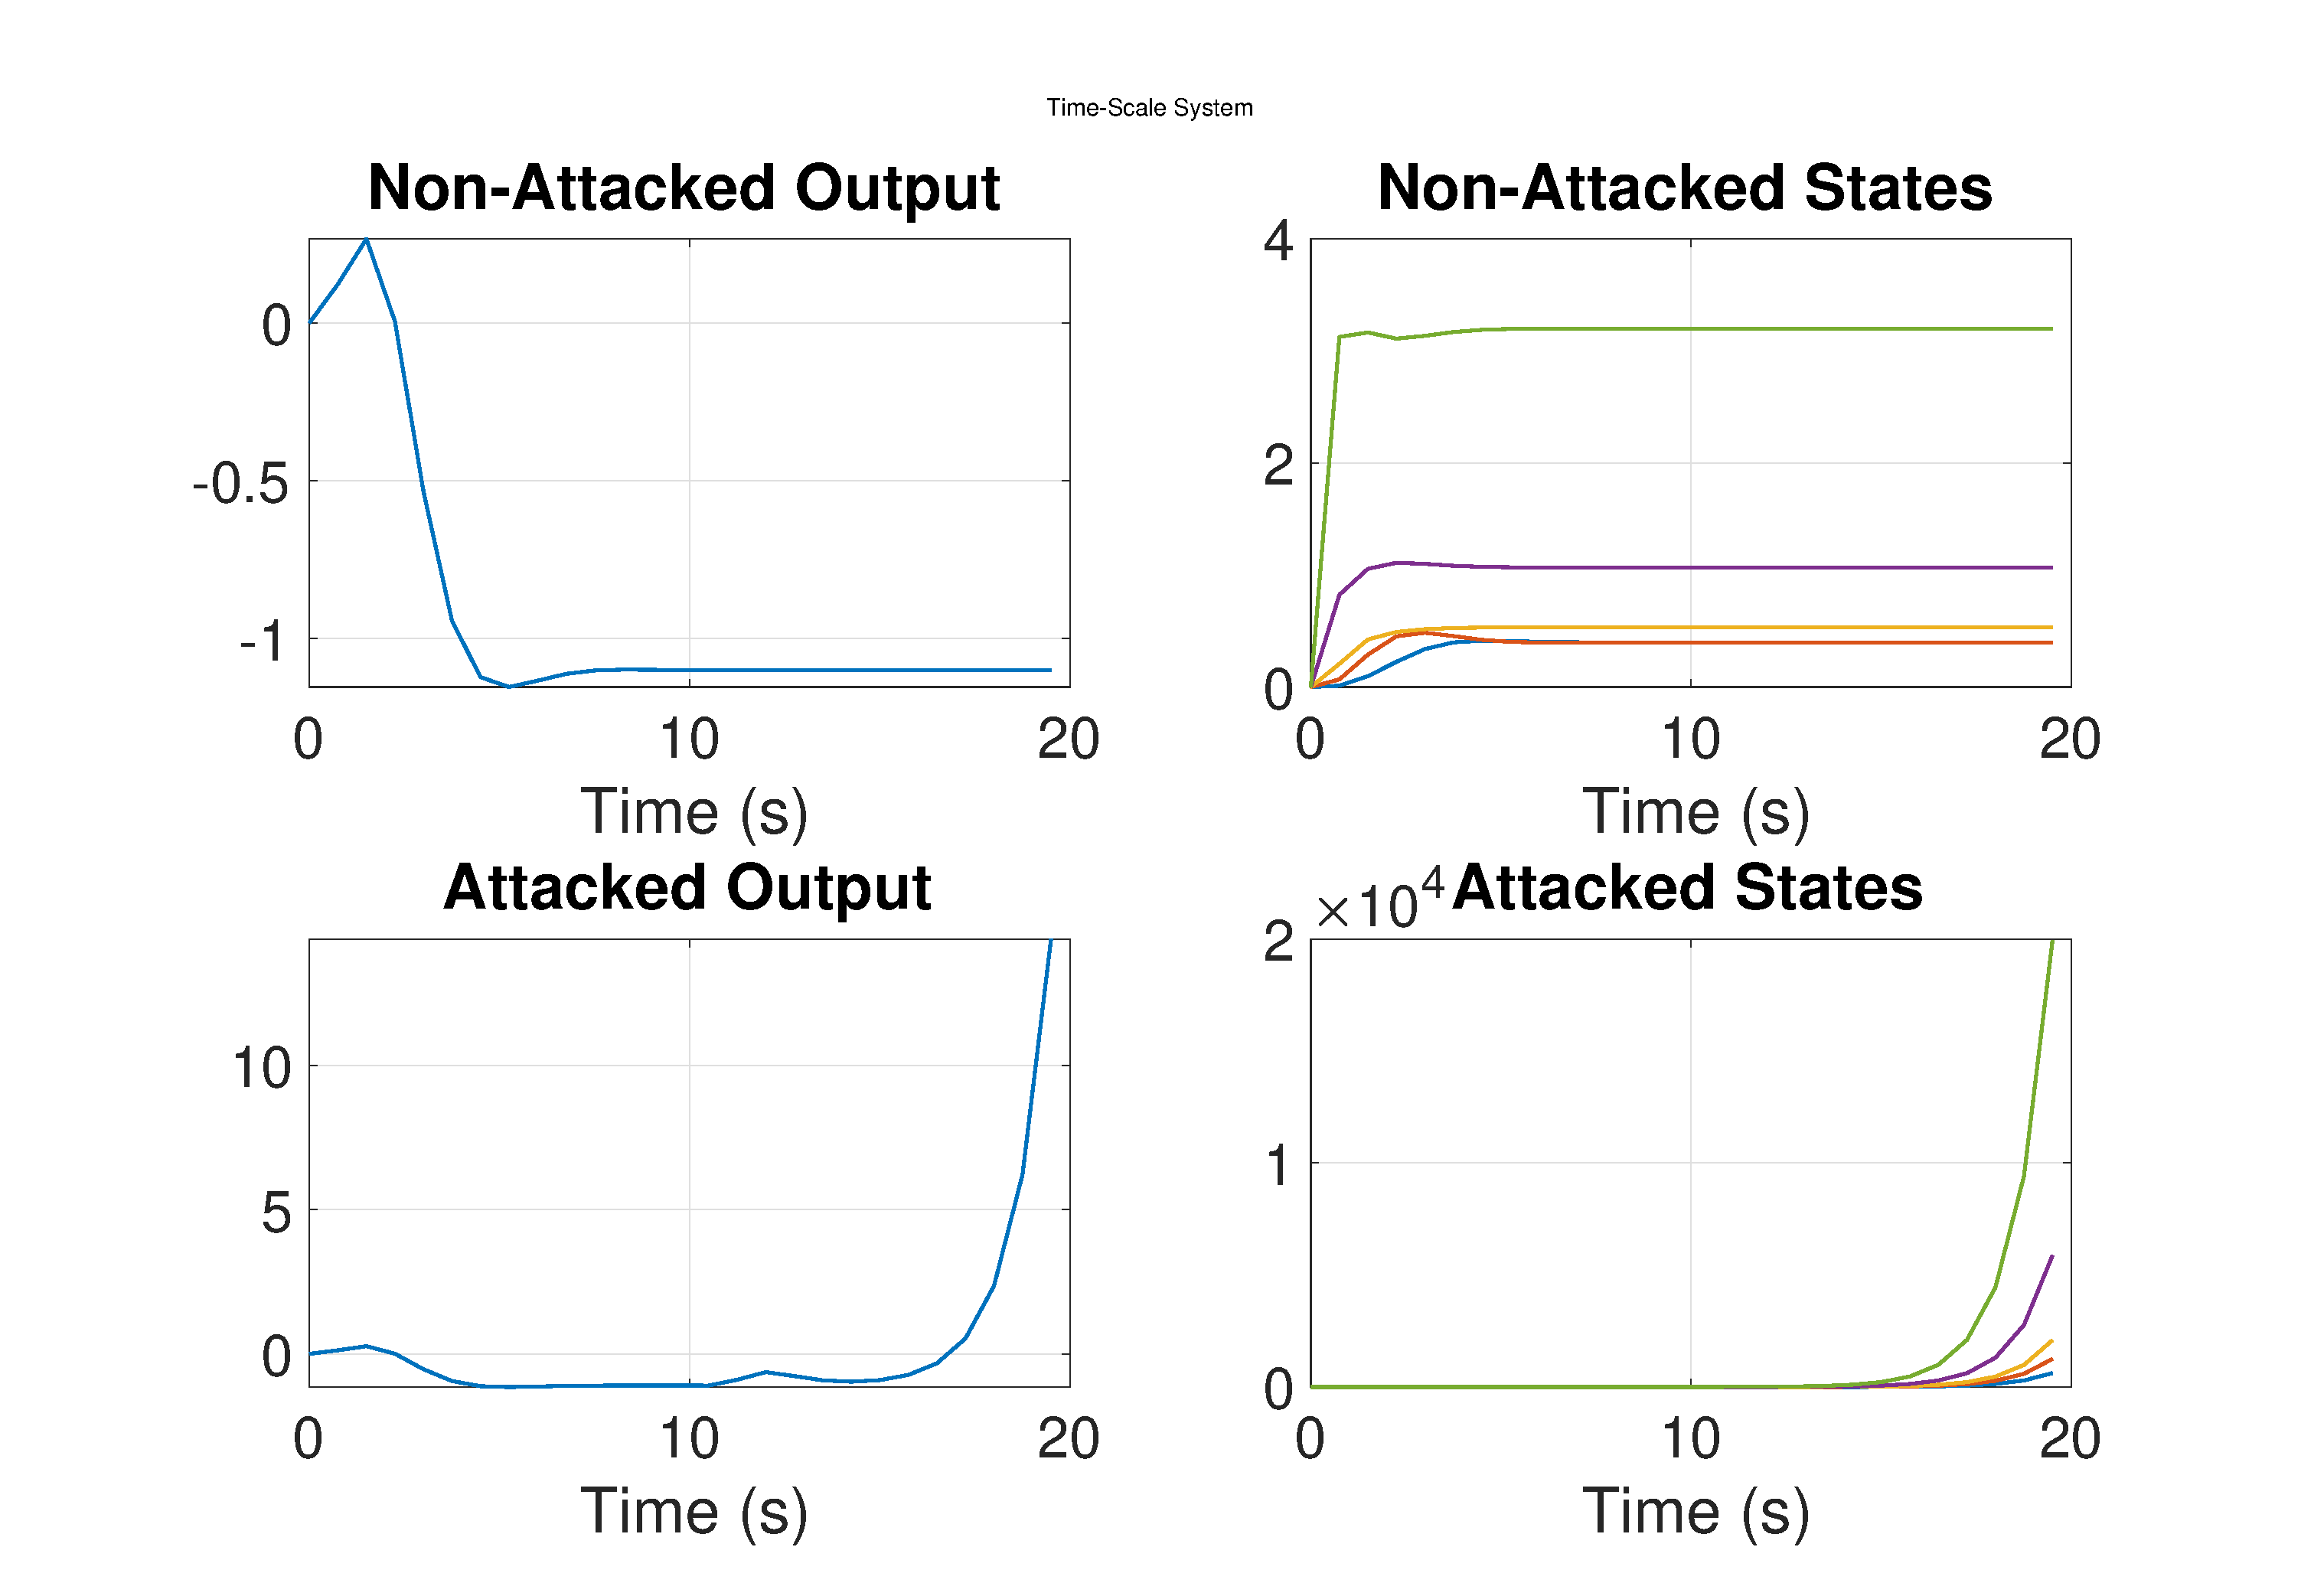
\includegraphics[width=\linewidth]{ts-system2}
        \caption{Time-scale system's observer with \(\mu=\SI{0.75}{\second}\).}%
        \label{fig:ts-system}
      \end{figure}
    \end{column}%
  \end{columns}
\end{slide}

% !TeX root = document.tex
% !TeX encoding = UTF-8 Unicode

\subsection{Partial Conclusion}%
\label{subsec:ts-conclusion}

\begin{slide}{Partial Conclusion}
  \begin{itemize}
    \item The formulation is straightforward, optimization based and extendable.
    \item The graininess \(\mu\) can change randomly to avoid attack vectors
          which may also affect the time-scale system. Better yet, techniques as
          the Game Theorie's Moving Target can give the best strategies to
          changing its value.
  \end{itemize}
\end{slide}


% !TeX root = document.tex
% !TeX encoding = UTF-8 Unicode

\section{Final Considerations}%
\label{sec:conclusion}

\begin{slide}{Future Works Perspective}
  \begin{itemize}
    \item Join the time-scale and functional-observer techniques.
    \item Make the resulting observer distributed.
  \end{itemize}
\end{slide}


\begin{slide}{}
  \usebeamercolor{frametitle}
  \vspace*{\fill}
  \begin{center}
    \textcolor{fg}{\Large{Merci pour votre attention.}}
  \end{center}
  \vspace*{\fill}
\end{slide}

\begin{slide}[allowframebreaks]{Referências}
  \nocite{*}
  \printbibliography{}
\end{slide}
\end{document}
